\documentclass[12pt,a4paper]{article}

% Packages
\usepackage[utf8]{inputenc}
\usepackage[T1]{fontenc}
\usepackage{amsmath,amssymb,amsfonts}
\usepackage{graphicx}
\usepackage{booktabs}
\usepackage{array}
\usepackage{multirow}
\usepackage{longtable}
\usepackage{float}
\usepackage{hyperref}
\usepackage{natbib}
\usepackage{geometry}
\usepackage{setspace}
\usepackage{enumitem}
\usepackage{xcolor}
\usepackage{tikz}
\usepackage{caption}
\usetikzlibrary{trees,positioning,arrows.meta}

\geometry{margin=1in}
\onehalfspacing

% Title
\title{\textbf{A Multiattribute Decision Analysis Framework for Selecting Synthetic Data Generation Methods: Balancing Fidelity, Privacy, Fairness, and Cost}}

\author{Michael Koo \and Alfonso Berumen}

\date{\today}

\begin{document}

\maketitle

\begin{abstract}
\noindent\textbf{Problem Statement:} Practitioners selecting a synthetic tabular data generation method face a multiattribute decision spanning distributional fidelity, privacy, fairness, and computational cost. The benchmarking literature increasingly reports performance matrices, but it typically stops short of translating metrics into decision-relevant guidance.

\noindent\textbf{Methodology:} We develop a decision-analytic framework that transforms method comparison into a structured value assessment. We construct a value-focused objectives hierarchy, define five primary measures (propensity AUC, DCR 5th percentile, TSTR F1 ratio, maximum subgroup utility gap, and total time), map measures to a common [0,1] value scale via single-dimensional value functions, and aggregate via an additive multiattribute value model. To represent heterogeneous practitioner preferences without requiring stakeholder elicitation, we specify swing weights via three stakeholder archetypes and examine robustness through sensitivity analysis. We further apply the decision-focused transformation of Dees et al.\ (2010) and quantify the value of additional benchmarking effort via a value of information analysis (Keisler 2004).

\noindent\textbf{Results:} We demonstrate the approach on the 2024 ACS PUMS person-level microdata for California ($N=35{,}000$ adult records), evaluating five representative method classes: Independent Marginals, Synthpop, CTGAN, a differentially private Bayesian network approach (PrivBayes-inspired), and GReaT.

\noindent\textbf{Practical Implications:} The framework shifts the question from ``which method is best'' to ``which method is best for your objectives,'' and provides an auditable template for organizations to (i) benchmark methods, (ii) make tradeoffs explicit, and (iii) identify when comprehensive evaluation is---and is not---worth the cost.

\vspace{0.5em}
\noindent\textbf{Keywords:} synthetic data generation, multiattribute utility theory, decision analysis, privacy-utility tradeoff, tabular data
\end{abstract}

\newpage
\tableofcontents
\newpage

%===============================================================================
\section{Introduction}
%===============================================================================

\subsection{The Business Practitioner's Decision Problem}

A data scientist at a public health agency needs to share demographic data with external researchers while protecting individual patient privacy. A survey methodologist at a public agency wants to create public-use microdata files that preserve complex, multivariate relationships. A machine learning engineer at a Fortune 500 company requires training data that accurately represents minority subgroups without exposing real individuals. Stakeholders will then use outputs from any of these sources to inform strategic decisions. Each faces a common, multi-faceted decision problem: (1) selecting the most appropriate synthetic data generation method, and (2) validating the resulting outputs before relying on them to make a major decision.

Organizations are increasingly relying on data analytics and Artificial Intelligence (AI), yet they face tension between leveraging data for innovation and protecting privacy (Harvard Business Review Analytic Services, 2021). Second, in domains from finance to healthcare, strict regulations (e.g.\ GDPR, CCPA) restrict the use and sharing of sensitive data (Harvard Business Review Analytic Services, 2021). Indeed, cross-border data transfers have become especially impacted as for example, the EU's Schrems II decision in 2020 invalidated the EU--US Privacy Shield framework, throwing into question how companies can legally move personal data overseas (International Association of Privacy Professionals, 2024). A third key driver is the need for faster experimentation and product development. Using synthetic data, firms can test algorithms, products, or scenarios quickly without waiting on slow or expensive data gathering cycles. For example, the health insurance company Humana found that synthetic data accelerated testing of new technologies: what used to take months of compliance checking with real data could be done in days with synthetic data, speeding up innovation (Harvard Business Review Analytic Services, 2021).

Synthetic data (SD) can be defined as artificially generated datasets that preserve the statistical properties of real data without exposing actual sensitive information (Eastwood, 2023). More clearly: ``Synthetic data is created rather than collected from real-world sources, with the aim of addressing varied challenges of data unavailability, scarcity, privacy or representativeness'' (World Economic Forum, 2025). Synthetic data is now used to do at least the following: (1) share and analyze sensitive data without exposing personally identifiable information (PII) (Giuffr\`{e} \& Shung, 2023), (2) augment sparse or imbalanced datasets to address data scarcity (Goyal \& Mahmoud, 2024), (3) simulate scenarios and stress tests, particularly for rare or costly events (WEKA, 2023), and (4) enable AI model or black-box Machine Learning (ML) model explainability through local ``what-if'' neighborhoods in methods such as LIME (Guidotti et al., 2023). At the same time, both journals and regulators emphasize the need for systematic evidence on utility and privacy trade-offs (Adams et al., 2025; El Emam et al., 2022). Estimates suggest that synthetic data usage likely exceeded 60\% for AI applications in 2024 (Zewe, 2025). Major technology companies including OpenAI, Apple, Microsoft, Google, Meta, and IBM are touting use of synthetic data for AI development and have highlighted their applications' capabilities in producing synthetic data for industry use (Kapania et al., 2025).

Practitioners view synthetic data as a valuable tool for tackling data scarcity, high collection costs, and privacy concerns, while also helping diversify datasets and evaluate model performance (Kapania et al., 2025). Even government agencies are taking note. In 2023 the U.S.\ Department of Homeland Security issued a call for solutions to generate synthetic data for machine learning in cases where real data is scarce or sensitive, highlighting the technology's strategic importance for public sector innovation (U.S.\ Department of Homeland Security, Science \& Technology Directorate, 2024). Yet, wide adoption presents what we see as a seemingly less acknowledged but important dilemma around best practices.

The core decision problem is which synthetic data approach to use and how to evaluate the resulting output. Synthetic data generation has quickly emerged as a promising approach for enabling data sharing, augmenting training datasets, and protecting privacy (Jordon et al., 2022). As a result, the methodological landscape has expanded rapidly, from statistical approaches such as sequential regression and non-parametric CART-based synthesis (Nowok et al., 2016) to more ``black-box'' deep learning methods including conditional generative adversarial networks (GANs) for tabular data (Xu et al., 2019) and transformer-based language models for realistic tabular data generation (Borisov et al., 2023), each embodying different assumptions about data structure and entailing distinct trade-offs.

Recent practitioner-focused research by Kapania et al.\ (2025) reveals that decision-makers in industry struggle with method selection and evaluation. Through 29 interviews with AI practitioners and responsible AI experts, they document pervasive challenges: practitioners lack rigorous validation protocols, rely on manual inspection that cannot scale easily, and have difficulty controlling synthetic data outputs to accurately represent underrepresented groups. Consider the following quote: ``Honestly, people just don't want to do [the validation] right now because of the urgency associated with everything'' (Kapania et al., 2025). We feel the authors identify a fundamental gap between the growing use of synthetic data and the development of best practices for its responsible deployment. This provides an opportunity for guidance driven by Decision Science as the domain has crossed both general decision-making and leveraging data analysis, primarily mathematical, for decision-making.

We propose that Decision Analysis approaches can provide a reliable framework to assess use cases for synthetic data. Trends in business, industry, government, and society have heightened attention to Data Analytics, Machine Learning, and AI methods while the influence of Decision Analysis has concurrently developed an increased focus in these methodological advances (Bier \& French, 2020). Additionally, there is a recognized overlap between data science methods for decision-making and the methods of expected-utility decision theory (Bier \& French, 2020). Here, we see an opportunity for both translation of synthetic data approaches and highlighting a clear relationship between decisions around synthetic data and decision theory; however for it to be relevant to practice we argue a framework requires a practitioner lens.

For a modern perspective, Phillips (2025) provides a practitioner-focused view on the ingredients for good decisions with structure including objectives, criteria, options, events, and outcomes and content to include consequences, preference values, trade-offs, probabilities, and risk attitude. Phillips (2025) further argues the process for creating any decision model includes: 1) considering context; 2) framing the problem; 3) providing content or information; 4) exploring results; and 5) agreeing on a way forward. The author finds these as the fifteen ingredients for Decision Technology but suggests the actual elements required to address a decision may be variable depending on the context (Phillips, 2025). More importantly, it is argued that a requisite decision model, described as a transitional object, must be sufficient in form and content to resolve a problem but should be seen as an art that requires social skills in interfacing with stakeholders (Phillips, 2025). Although we cannot directly facilitate organizational synthetic data decisions to co-create requisite models, fully capturing nuances like data usage, evaluation, and real-world consequences, a streamlined methodology offers practitioners a practical, structured alternative.

\subsection{Overview of Current Business Applications}

Across business and data science domains, synthetic data is increasingly used to mitigate data scarcity, high collection costs, and privacy or regulatory constraints, with practitioners highlighting its value for bias reduction, privacy protection, and model development or scoring (Kapania et al., 2025; Eastwood, 2023). Organizations generate artificial datasets that mirror real ones so they can incorporate data-driven decision-making despite strict regulations or sparse data environments, a trend reflected in forecasts that a large share of business AI training data will be synthetically generated (Eastwood, 2023). The World Economic Forum recently released a briefing paper titled ``Synthetic Data: The New Data Frontier'' which explicitly suggests synthetic data enables robust analytics to facilitate data-driven decision-making (World Economic Forum, 2025).

Synthetic data can be created in multiple formats, such as structured tabular records, time-series, text, images, video, and graphs, enabling teams to analyze patterns, build algorithms, and test software while keeping sensitive details confidential (Giuffr\`{e} \& Shung, 2023). Tabular synthetic data, in particular, is the dominant format in business settings because most enterprise information systems store customer records, transactions, and operational metrics in structured, table-like databases, making it the natural substrate for analytics and AI in finance, retail, and other process areas and functions. For example, datasets or databases that involve people are typically tabular in format in which each record corresponds to a person such as a customer or patient, and the columns represent characteristics such as demographics or activity. Tabular data in its cleanest form can further be described as structured data that is ready for mathematical or statistical analysis.

Because of this ubiquity, synthetic data research has placed particular emphasis on tabular data generation methods. For example, Shi et al.\ (2025) describe tabular data as ``the most prevalent and important data formats in real-world applications such as healthcare, finance, and education,'' underscoring its importance in business contexts. Similarly, Pathare et al.\ (2023) evaluate multiple synthetic tabular generation techniques across balanced and imbalanced datasets, reflecting how central structured, row-and-column data are to applied machine learning. Reviews of generative modeling tools for tabular data (Figueira et al., 2022) and systematic surveys of evaluation approaches (Shi et al., 2025) further highlight that business-critical datasets are typically stored and exchanged in tabular form, reinforcing why synthetic methods for this format dominate both academic and practitioner attention.

In marketing, synthetic data supports customer analytics, pricing, and targeting while protecting individual-level information. For example, Anand and Lee (2023) show that a shared GAN-based generator can produce synthetic customer records that preserve key behavioral patterns, allowing external partners to optimize price markups and targeting decisions with performance close to models trained on real data. Other work using Nielsen scanner data demonstrates that Bayesian synthetic data can maintain accurate estimates of elasticities and promotion effects, avoiding the aggregation bias and information loss that occur with traditional anonymization methods such as heavy aggregation or addition of noise (Schneider, Jagpal, \& Gupta, 2018).

In human resources and people analytics, synthetic data is promoted as a way to reconcile innovation with privacy, trust, and legal compliance when handling sensitive employee records (SHRM, 2024a, 2024b, 2024c, 2025). HR and people analytics teams use synthetic workforce datasets to explore retention drivers, DEI outcomes, or performance patterns, collaborate with external vendors, and prototype predictive models without exposing real employees' data.

Healthcare has likewise become a leading domain: hospitals and researchers employ synthetic electronic health records and medical images to enable privacy-preserving research, algorithm training, and patient profiling while meeting HIPAA and ethical requirements, as evidenced by deployments such as Washington University's use of MDClone for COVID-19 studies and broader analyses of synthetic health data for personalized medicine, public health, and regulatory evaluation.

In finance and other regulated sectors, banks and insurers employ synthetic transaction data for fraud detection, anti-money laundering (AML), and risk modeling, while manufacturing, telecom, automotive, and robotics organizations use synthetic data and scenarios to support quality control, predictive maintenance, cyberattack simulation, and training of autonomous systems (Harvard Business Review Analytic Services, 2021; NayaOne, 2025; AIMultiple, 2025).

In short, synthetic data's appeal spans virtually every data-reliant domain, including healthcare, finance, automotive, retail, manufacturing, insurance, and beyond. Organizations therefore need guidance on best practices as practitioners and regulators work to establish standards amid rapid industry adoption.

\subsection{Limitations of Current Literature}

The synthetic data evaluation literature has grown substantially, yet it offers limited decision support. Kaabachi et al.\ (2025), in a comprehensive review of 73 studies on privacy and utility metrics in medical synthetic data, find that while 95\% of studies evaluate utility and 82\% cite privacy as motivation, only 46\% actually assess privacy. These researchers' taxonomy identifies broad utility (statistical fidelity), narrow utility (task-specific performance), fairness, and privacy attack metrics---yet they conclude there is no consensus on standardized approach for systematically evaluating privacy and utility. As an additional note, utility in this domain refers to the usefulness of synthetic data which can be qualified in different ways, not to be confused with the formal definition of utility in the decision science domain.

Stoian et al.\ (2025) provide an extensive survey explicitly framed as a ``user guide'' for practitioners navigating the synthetic data space, organizing requirements around utility, alignment with domain knowledge, fidelity, and privacy. With respect to utility they suggest, ``Synthetic data should yield similar predictive performance to real data when used to train machine learning (ML) models for the same task, such as classification or regression'' whereas alignment refers to alignment with user-provided domain-specific knowledge, fidelity refers to the preservation of the statistical properties of the original data, and privacy as protecting against the re-identification of individuals (Stoian et al.\ 2025). Hernandez et al.\ (2025) offers a comprehensive evaluation framework applied to five generative models across three medical datasets, finding that simpler statistical models achieve better fidelity (based on metrics on mathematical metrics), and utility (based on prediction metrics), while complex deep learning models provide lower privacy risk (based on identification computations)---a tradeoff with no obvious resolution.

These contributions advance our understanding of what to measure, but they do not tell practitioners how to decide. Benchmark studies commonly report performance matrices with metrics like KS statistics without application-specific decision thresholds or clear guidance on fidelity-privacy tradeoffs, leaving practitioners to interpret raw numbers. The FCA, ICO, and Alan Turing Institute's 2023 roundtable on synthetic data validation identifies utility, fidelity, and privacy as key barriers and calls for step-by-step frameworks and industry standards to support adoption.

\subsection{A Decision Analysis Approach to Synthetic Data}

We propose treating the choice of synthetic data methods as a multiattribute decision problem addressed with the tools of decision analysis. Drawing on the value-focused thinking (VFT) paradigm (Keeney, 1992), we start by articulating the fundamental objectives practitioners care about---the purposes synthetic data must serve---rather than anchoring on existing methods or available packages. On this foundation, we develop a formal multiattribute value model that converts raw performance metrics into preference-weighted scores, yielding practitioner-relevant assessments of each method.

While multiattribute decision analysis literature is mature, our approach draws on three foundational Decision Analysis papers that provide methodological templates and practitioner examples. Butler et al.\ (2005) demonstrate structuring complex technology selection via objectives hierarchy, swing weights, and sensitivity analysis. Keisler (2004) shows assessing the value of information in portfolios. Dees, Dabkowski, and Parnell (2010) develop discriminatory value transformations. Integrating these, we propose a framework with: (1) objectives hierarchy from practitioner values, (2) single-dimensional value functions, (3) swing weights derived through stakeholder archetypes representing distinct preference profiles, and (4) decision-focused transformation revealing where methods truly differ.

\subsection{Contributions and Paper Organization}

This paper makes three contributions. First, we develop the first multiattribute decision analysis framework for synthetic data method selection (VF-SDSF: Value-Focused Synthetic Data Selection Framework), integrating value-focused objectives hierarchy, single-dimensional value functions, stakeholder archetypes, decision-focused transformation, and value of information analysis. The framework is domain-general and can be applied to any tabular data context, providing practitioners systematic, auditable guidance for method selection tailored to organizational priorities.

Second, we demonstrate framework feasibility through proof-of-concept application to California American Community Survey Public Use Microdata Sample ($N=35{,}000$ adult records), evaluating five generation methods across five primary value measures (fidelity, privacy, utility, fairness, efficiency). This demonstrates the framework is implementable and reveals preference-dependent method rankings---insights not apparent from raw metric inspection. While our specific empirical findings are dataset-specific, they show that optimal method choice depends critically on practitioner objectives, with no method dominating across all criteria.

Third, we conduct value of information analysis identifying when comprehensive benchmarking is---and is not---worth the investment, providing practical decision rules for resource allocation in method evaluation. While our empirical findings are specific to ACS PUMS, the framework provides a reusable template for organizations to systematically evaluate methods in their own context.

The paper proceeds as follows. Section 2 defines the decision context and stakeholder archetypes. Section 3 develops the objectives hierarchy and value measures. Section 4 describes the alternative generation methods. Section 5 presents the value-focused multiattribute model. Section 6 reports our empirical application to ACS PUMS data. Section 7 applies the decision-focused transformation. Section 8 conducts the value of information analysis. Section 9 examines sensitivity of results to assumptions and model specifications. Section 10 discusses framework generalizability, practical implications, and limitations.

%===============================================================================
\section{Decision Context}
%===============================================================================

\subsection{The Stakeholder}

We conceptualize the decision maker as a practitioner who must generate synthetic tabular data for a specified purpose. This encompasses data scientists preparing public-use files, researchers augmenting training data, privacy officers enabling data sharing, and organizations producing data for testing, education, or training purposes. Different stakeholders may hold different preferences---for example, a privacy officer might weigh privacy preservation more heavily than a machine learning engineer optimizing model predictive performance. However, all face the same fundamental decision problem; what varies is the decision context (e.g., why now, who decides, scope, constraints such as budget, regulations, or data availability).

\textbf{Framework Context}: While our empirical demonstration uses publicly available ACS PUMS data (necessary for reproducible research), the framework is designed for practitioners working with private, sensitive datasets where method selection has direct privacy, utility, and fairness implications. Organizations applying this framework to private healthcare, financial, or HR data face different privacy constraints than our demonstration context but can use the same systematic evaluation structure.

To accommodate practitioner heterogeneity while maintaining tractability, we define three stakeholder archetypes representing distinct but plausible preference profiles:

\begin{description}
    \item[Privacy-First Practitioner:] Works in healthcare, finance, or government where regulatory compliance and individual protection are paramount. Willing to sacrifice some fidelity and utility for strong privacy guarantees.
    
    \item[Utility-First Practitioner:] Machine learning engineer focused on model training. Needs synthetic data that supports equivalent predictive performance. Privacy concerns are secondary (perhaps already addressed through access controls).
    
    \item[Balanced Practitioner:] General-purpose data scientist seeking reasonable performance across all dimensions. No single objective dominates. Represents the ``typical'' user without extreme preferences.
\end{description}

The decision maker may vary, but similarly experiences ``a sense of unease'' about the present situation---uncertainty about which method will best serve their needs---and seeks a model to ``explore possible futures'' before committing to a choice (Phillips, 2025). The value-focused multiattribute model serves as what Phillips (2025) calls a ``transitional object,'' where the requisite decision model makes preferences explicit, reduces anxiety, and enables systematic evaluation of alternatives.

\subsection{The Decision}

The decision can be stated formally: given (1) an original dataset with known characteristics, (2) an intended use case specifying downstream analytical tasks, and (3) constraints and considerations on privacy protection and computational resources, select the synthetic data generation method that maximizes value across relevant objectives.

This framing makes explicit that method selection is context-dependent. A method optimal for generating medical records with strong privacy requirements may differ from one optimal for augmenting a small training dataset where fidelity to multivariate structure dominates. The multiattribute decision analysis framework accommodates this heterogeneity through adjustable weights rather than seeking a universally ``best'' method.

\subsection{Key Uncertainties}

Three sources of uncertainty complicate the decision. First, downstream task performance is unknown at the time the synthetic data is generated. The synthetic data will be used for analyses not yet fully specified, and its utility for those tasks cannot be directly observed until they occur. Second, privacy risk depends on attack sophistication. A dataset resistant to current membership inference attacks may become vulnerable as attack methods advance. Third, dataset characteristics interact with method performance in ways that may not transfer across domains. A method that excels on census data may underperform on electronic health records.

Following Butler et al.\ (2005), we model these uncertainties implicitly through the performance estimates rather than constructing explicit probability distributions over future states. Scoring and sensitivity analysis is recommended over probabilistic methods when probabilities are unavailable or less known (NIST, 1995). Due to the individualized use cases, unknown downstream tasks, and evolving privacy attack sophistication, we argue that this approach matches decision problems around synthetic data. This approach maintains tractability while acknowledging that value estimates represent expected performance under uncertainty.

%===============================================================================
\section{Objectives Hierarchy and Value Measures}
%===============================================================================

\subsection{Values}

Consistent with Keeney (1992), practitioner values emphasize privacy protection alongside downstream utility, addressing data scarcity, competitive advantage, and equitable representation of groups (Kapania et al., 2025; Kaabachi et al., 2025; Vallevik et al., 2024). These values, derived from surveys of synthetic data users and empirical research, guide the identification of the fundamental objectives below.

\subsection{Fundamental Objectives Hierarchy}

We decompose these values into five fundamental objectives, each grounded in practitioner values.

\begin{enumerate}
    \item \textbf{Distributional Fidelity}: Captures whether synthetic data preserves the statistical properties of real data. Stoian et al.\ (2025) distinguish this from utility, defining fidelity as ``statistical similarity'' encompassing marginal distributions, correlations, and higher-order structure. Kaabachi et al.\ (2025) identify ``broad utility'' as the most frequently assessed dimension, appearing in 95\% of studies reviewed. Fidelity serves as a necessary---though not sufficient---condition for downstream usefulness.
    
    \item \textbf{Privacy Preservation}: Reflects minimal risk of re-identification or sensitive attribute disclosure. Despite 82\% of studies citing privacy as a motivation for using synthetic data, only 46\% evaluate it empirically (Kaabachi et al., 2025). Privacy measures include membership inference attack success, attribute inference risk, and distance-to-closest-record metrics. Hernandez et al.\ (2025) find privacy and fidelity directly at odds---methods achieving high fidelity tend to provide weaker privacy guarantees.
    
    \item \textbf{Downstream Utility}: Measures whether synthetic data supports intended analytical tasks. The standard protocol, train-on-synthetic-test-on-real (TSTR), trains models on synthetic data and evaluates on held-out real data. Kaabachi et al.\ (2025) term this ``narrow utility,'' distinguishing it from distributional fidelity. A dataset may preserve marginal distributions perfectly yet fail to support predictive modeling if it corrupts the relationships relevant to the prediction task.
    
    \item \textbf{Fairness and Equity}: Captures equitable quality across demographic or other key characteristic subgroups. Kaabachi et al.\ (2025) find that while broad utility was noted in 153 evaluation instances, only 3 instances addressed fairness, identifying fairness as severely underexplored. Kapania et al.\ (2025) document practitioner struggles with ``generating data that accurately depict underrepresented groups.'' Fairness and Equity measures assess whether synthetic data maintains representation quality and downstream model performance across demographic groups.
    
    \item \textbf{Operational Efficiency}: Encompasses computational cost, implementation complexity, and scalability. Hernandez et al.\ (2025) acknowledge a gap in their framework: ``lacks evaluation metrics for training time and resource usage.'' Kapania et al.\ (2025) document that practitioners value methods enabling efficient iteration, particularly when validation relies on manual inspection. For resource-constrained practitioners, a method requiring GPU clusters may be infeasible regardless of performance.
\end{enumerate}

Figure~\ref{fig:hierarchy} presents the complete objectives hierarchy visually.

\begin{figure}[htbp]
\centering
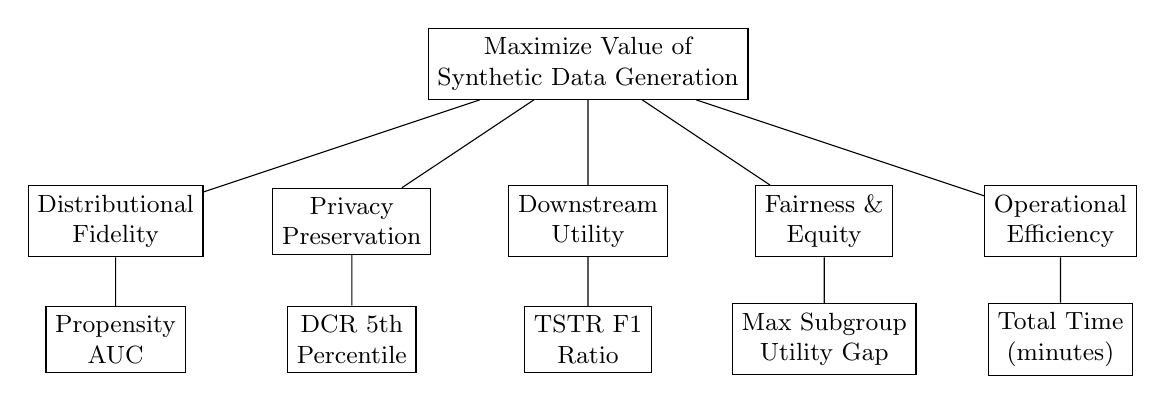
\begin{tikzpicture}[
    level 1/.style={sibling distance=3cm, level distance=2cm},
    level 2/.style={sibling distance=2cm, level distance=1.5cm},
    every node/.style={rectangle, draw, align=center, font=\small}
]
\node {Maximize Value of\\Synthetic Data Generation}
    child {node {Distributional\\Fidelity}
        child {node {Propensity\\AUC}}}
    child {node {Privacy\\Preservation}
        child {node {DCR 5th\\Percentile}}}
    child {node {Downstream\\Utility}
        child {node {TSTR F1\\Ratio}}}
    child {node {Fairness \&\\Equity}
        child {node {Max Subgroup\\Utility Gap}}}
    child {node {Operational\\Efficiency}
        child {node {Total Time\\(minutes)}}};
\end{tikzpicture}
\caption{Objectives hierarchy for synthetic data generation method selection. The hierarchy decomposes the fundamental objective into five measurable attributes aligned with practitioner values.}
\label{fig:hierarchy}
\end{figure}

\subsection{Attributes and Measures}

Each objective is operationalized through attributes meeting Keeney and Gregory's (2005) criteria: unambiguous, comprehensive, direct, operational, and understandable. We selected measures based on three practitioner-focused criteria: (1) alignment with established evaluation frameworks in the synthetic data literature, (2) feasibility of computation without requiring external resources (e.g., access to attackers), and (3) coverage of the objective's essential dimensions.

\subsubsection{Fidelity Measures}

\textbf{Primary Measure: Propensity Score AUC.} We train a classifier to distinguish real from synthetic records. An AUC near 0.5 indicates synthetic data is indistinguishable from real data, representing perfect fidelity. An AUC of 1.0 indicates the classifier perfectly distinguishes synthetic from real, representing zero fidelity. This measure captures overall distributional similarity in a single metric and has been validated in prior synthetic data evaluation studies (Hernandez et al., 2025).

\textbf{Secondary Measures:} Average Kolmogorov-Smirnov (KS) statistic for continuous variables assesses marginal distribution preservation, with lower values indicating better performance. Average Total Variation Distance (TVD) for categorical variables similarly captures marginal fidelity for discrete attributes.

\subsubsection{Privacy Measures}

\textbf{Primary Measure: Distance to Closest Record (DCR) 5th Percentile.} DCR measures the minimum distance from each synthetic record to its nearest training record, with the 5th percentile capturing the ``worst-case'' synthetic records most similar to training data. Higher DCR values indicate better privacy (synthetic records are further from training data).

\textbf{Methodological Note:} We initially planned to use membership inference attack success rate as the primary privacy measure. However, during validation experiments, we found that the membership inference attack classifier achieved AUC $\approx$ 0.50 on real data (unable to distinguish training members from non-members), rendering the measure uninformative for this dataset. DCR provides a direct measure of memorization risk without requiring a functioning attack classifier.

\subsubsection{Utility Measures}

\textbf{Primary Measure: TSTR F1 Ratio.} We train a classifier on synthetic data and evaluate on held-out real test data. The TSTR F1 ratio compares F1 score when trained on synthetic versus real data, with a ratio near 1.0 indicating synthetic data supports equivalent model quality. Our prediction task is binary classification of high income (annual personal income $>$ \$50,000).

\textbf{Secondary Measure:} TSTR AUC Ratio follows the same computation, replacing F1 with AUC.

\subsubsection{Fairness Measures}

\textbf{Primary Measure: Maximum Subgroup Utility Gap.} We compute TSTR F1 ratio separately for each demographic subgroup and report the maximum absolute difference between any subgroup's ratio and the overall ratio. This measure captures whether synthetic data quality varies systematically across demographic groups.

\textbf{Subgroup Definition:} Race (RAC1P variable), collapsed to five categories: White, Black, Asian, Hispanic, and Other. We require a minimum subgroup size of $n \geq 100$ in the test set for inclusion in the gap calculation.

\subsubsection{Efficiency Measures}

\textbf{Primary Measure: Total Time (Minutes).} Wall-clock time for training the generative model plus generating the synthetic dataset. This captures the practical computational burden practitioners face.

Table~\ref{tab:measures} summarizes the measure specifications.

\begin{table}[htbp]
\centering
\caption{Value Measure Specifications}
\label{tab:measures}
\begin{tabular}{@{}llll@{}}
\toprule
\textbf{Objective} & \textbf{Primary Measure} & \textbf{Scale Direction} & \textbf{Secondary Measures} \\
\midrule
Fidelity & Propensity Score AUC & Lower is better (closer to 0.5) & Avg KS, Avg TVD \\
Privacy & DCR 5th Percentile & Higher is better & Membership Inference \\
Utility & TSTR F1 Ratio & Higher is better (closer to 1.0) & TSTR AUC Ratio \\
Fairness & Max Subgroup Utility Gap & Lower is better (closer to 0) & --- \\
Efficiency & Total Time (minutes) & Lower is better & --- \\
\bottomrule
\end{tabular}
\end{table}

%===============================================================================
\section{Alternatives: Synthetic Data Generation Methods}
%===============================================================================

Tabular data dominates business applications (Shi et al., 2025). We evaluate five methods spanning statistical approaches, deep learning methods, differentially private techniques, and language model-based approaches---a comprehensive representation of the current methodological landscape (Shi et al., 2025; Hernandez et al., 2025).

\subsection{Trivial Baseline}

\textbf{Independent Marginals} samples each column independently from its empirical marginal distribution. This approach preserves marginals perfectly but destroys all correlations between variables. We include this method as a floor for comparison, defining the worst acceptable performance ($x_{\text{worst}}$) for fidelity, utility, and fairness measures. Any practical method should substantially outperform this baseline.

\subsection{Statistical Methods}

\textbf{Synthpop} (Nowok, Raab, \& Dibben, 2016) implements sequential CART-based synthesis. Variables are synthesized one at a time conditional on previously synthesized variables, with conditional distributions estimated via classification and regression trees. This approach handles mixed data types naturally and provides interpretable synthesis decisions. It remains widely used in official statistics and survey methodology. We use the R package \texttt{synthpop} with default parameters (method = ``cart'', cart.minbucket = 5).

\subsection{Deep Learning Methods}

\textbf{CTGAN} (Xu et al., 2019) adapts generative adversarial networks for tabular data. Key innovations include mode-specific normalization for continuous variables, conditional generation to address class imbalance, and training-by-sampling to ensure all categories are represented. CTGAN has become a standard benchmark in the synthetic data literature. We use the Python \texttt{sdv} library with default parameters (epochs = 300).

\subsection{Differentially Private Methods}

\textbf{DP Bayesian network (PrivBayes-inspired).} PrivBayes (Zhang et al., 2014) is a differentially private Bayesian network approach for private data release. In our implementation, we use the Python \texttt{DataSynthesizer} library's correlated-attribute mode as a PrivBayes-inspired DP Bayesian network synthesis procedure, with privacy budget $\varepsilon = 1.0$ and Bayesian network degree = 2.

\subsection{Language Model Methods}

\textbf{GReaT} (Borisov et al., 2023) fine-tunes pretrained language models on textual representations of tabular data. Each row is converted to a natural language sentence, the language model is fine-tuned, and new rows are generated via text completion. This approach leverages the world knowledge and pattern recognition capabilities of large language models. We use the Python \texttt{be-great} library with distilgpt2 as the base model and epochs = 50.

Table~\ref{tab:methods} summarizes the method specifications.

\begin{table}[htbp]
\centering
\caption{Synthetic Data Generation Method Specifications}
\label{tab:methods}
\begin{tabular}{@{}llll@{}}
\toprule
\textbf{Method} & \textbf{Type} & \textbf{Implementation} & \textbf{Key Parameters} \\
\midrule
Independent Marginals & Trivial baseline & Custom & --- \\
Synthpop & Statistical & R \texttt{synthpop} & method=``cart'', minbucket=5 \\
CTGAN & Deep learning (GAN) & Python \texttt{sdv} & epochs=300 \\
DP BN (PrivBayes-inspired) & Differentially private & Python \texttt{DataSynthesizer} & $\varepsilon=1.0$, degree=2 \\
GReaT & Language model & Python \texttt{be-great} & distilgpt2, epochs=50 \\
\bottomrule
\end{tabular}
\end{table}

%===============================================================================
\section{Multiattribute Value Model}
%===============================================================================

\subsection{Model Structure}

Following Keeney and Raiffa (1976), we employ an additive multiattribute value model. Let $x_{ij}$ denote the performance of method $j$ on measure $i$. The overall value of method $j$ is:

\begin{equation}
V(\text{method}_j) = \sum_i w_i \times v_i(x_{ij})
\end{equation}

where $w_i$ is the swing weight for objective $i$ (with $\sum w_i = 1$) and $v_i(x)$ is the single-dimensional value function mapping performance on measure $i$ to a $[0,1]$ preference scale.

\textbf{Preferential Independence Assumption}: The additive form assumes preferential independence across objectives: that preferences over one objective do not systematically depend on levels achieved on other objectives (Keeney \& Raiffa, 1976). This is a standard assumption in multiattribute decision analysis, enabling tractable value aggregation while maintaining transparency.

\subsection{Single-Dimensional Value Functions}

For each measure, we specify a value function $v_i(x) \in [0,1]$ where 0 represents the worst acceptable performance and 1 represents the best achievable performance. We employ benchmark-relative anchoring, where:
\begin{itemize}
    \item $x_{\text{best}}$: Best performance observed across all methods (excluding Independent Marginals for fidelity/utility/fairness)
    \item $x_{\text{worst}}$: Performance of Independent Marginals baseline (for fidelity, utility, fairness) OR reasonable worst-case (for privacy, efficiency)
\end{itemize}

Linear scaling is used for all objectives except operational efficiency:

\textbf{Fidelity (Propensity Score AUC):}
\begin{equation}
v_{\text{fidelity}}(x) = \frac{x_{\text{worst}} - x}{x_{\text{worst}} - 0.50}
\end{equation}

\textbf{Privacy (DCR 5th Percentile):}
\begin{equation}
v_{\text{privacy}}(x) = \frac{x - x_{\text{worst}}}{x_{\text{best}} - x_{\text{worst}}}
\end{equation}

\textbf{Utility (TSTR F1 Ratio):}
\begin{equation}
v_{\text{utility}}(x) = \frac{x - x_{\text{worst}}}{1.0 - x_{\text{worst}}}
\end{equation}

\textbf{Fairness (Max Subgroup Utility Gap):}
\begin{equation}
v_{\text{fairness}}(x) = \frac{x_{\text{worst}} - x}{x_{\text{worst}}}
\end{equation}

\textbf{Efficiency (Total Time):}
\begin{equation}
v_{\text{efficiency}}(x) = 1 - \frac{\log(x / x_{\text{best}})}{\log(480 / x_{\text{best}})}
\end{equation}

The logarithmic form for efficiency reflects that going from 1 minute to 10 minutes is more consequential than going from 100 minutes to 110 minutes---a reasonable representation of practitioner sensitivity to time costs.

\subsection{Swing Weight Derivation}

Swing weights reflect the relative importance of moving from worst to best performance on each objective. Rather than eliciting weights from a specific expert panel---which would limit generalizability---we derive weights through stakeholder archetypes representing distinct but plausible preference profiles, supplemented by extensive sensitivity analysis across plausible ranges.

Table~\ref{tab:weights} presents the swing weights for each stakeholder archetype.

\begin{table}[htbp]
\centering
\caption{Swing Weights by Stakeholder Archetype}
\label{tab:weights}
\begin{tabular}{@{}lccc@{}}
\toprule
\textbf{Objective} & \textbf{Privacy-First} & \textbf{Utility-First} & \textbf{Balanced} \\
\midrule
Fidelity & 0.25 & 0.30 & 0.25 \\
Privacy & 0.45 & 0.10 & 0.25 \\
Utility & 0.15 & 0.40 & 0.25 \\
Fairness & 0.10 & 0.10 & 0.15 \\
Efficiency & 0.05 & 0.10 & 0.10 \\
\midrule
\textbf{Total} & 1.00 & 1.00 & 1.00 \\
\bottomrule
\end{tabular}
\end{table}

We emphasize these are illustrative weights for demonstration. Section 9 presents extensive sensitivity analysis examining how conclusions change across plausible weight ranges, enabling practitioners to identify results robust to their specific preference profiles.

%===============================================================================
\section{Empirical Application: ACS PUMS Case Study}
%===============================================================================

\subsection{Data Description}

We apply the framework to the American Community Survey (ACS) Public Use Microdata Sample (PUMS), a standard benchmark in synthetic data research that reflects real-world complexity including mixed variable types, class imbalance, and demographic diversity. The ACS provides detailed demographic, economic, and housing information for over 3.5 million individuals annually, making it ideal for evaluating generation methods across diverse data characteristics.

Our analysis uses $N = 35{,}000$ adult records randomly sampled from the 2024 1-Year ACS PUMS California person file. We select this dataset for several reasons: (1) it is publicly available, enabling full reproducibility; (2) it contains person-level records with demographic attributes suitable for fairness analysis; (3) it includes mixed variable types (continuous and categorical) that challenge generation methods; and (4) it avoids the overuse of standard machine learning benchmark datasets (e.g., UCI datasets) that may already contain synthetic records.

\subsubsection{Variable Selection}

\textbf{Continuous Variables (2):}
\begin{itemize}
    \item Age (AGEP): Age of person
    \item Income (PINCP): Total person's income
\end{itemize}

\textbf{Categorical Variables (6):}
\begin{itemize}
    \item Sex (SEX): 2 categories
    \item Race (RAC1P + HISP): recoded with Hispanic override, 5 categories
    \item Education (SCHL): Educational attainment recoded to 5 levels
    \item Marital Status (MAR): 5 categories
    \item Employment Status (ESR): 6 categories
    \item Nativity (POBP): US-born vs.\ foreign-born, 2 categories
\end{itemize}

\textbf{Target Variable:} HIGH\_INCOME = 1 if PINCP $>$ \$50,000, else 0 (binary classification)

\subsubsection{Data Preprocessing}

We apply the following preprocessing steps:
\begin{enumerate}
    \item Filter to adults (AGEP $\geq$ 18)
    \item Restrict to records with valid income values (PINCP present)
    \item Recode categorical variables:
    \begin{itemize}
        \item SCHL: collapse to 5 levels ($<$HS, HS, Some college, Bachelor's, Graduate)
        \item RAC1P + HISP: collapse to 5 categories (White, Black, Asian, Hispanic, Other)
        \item POBP: recode to US-born vs.\ foreign-born
    \end{itemize}
    \item Construct the binary target: HIGH\_INCOME = 1 if PINCP $>$ 50,000, else 0
    \item Randomly sample to $N = 35{,}000$ (if more eligible records are available)
\end{enumerate}

\textbf{Note on Survey Weights:} We do not incorporate ACS survey weights in this analysis. While survey weights are important for population inference, our focus is on demonstrating the decision framework rather than producing population-representative synthetic data. This limitation is noted in Section 10.

\subsubsection{Data Partitioning}

\begin{table}[htbp]
\centering
\begin{tabular}{@{}llll@{}}
\toprule
\textbf{Partition} & \textbf{Proportion} & \textbf{Size} & \textbf{Purpose} \\
\midrule
Training & 70\% & 24,500 & Train generative models \\
Test & 30\% & 10,500 & TSTR evaluation (never seen by generators) \\
\bottomrule
\end{tabular}
\end{table}

\textbf{Critical:} The test set is held out entirely. Synthetic data is generated from the training set only. TSTR models are trained on synthetic data and evaluated on the real test set.

\subsection{Experimental Protocol}

We follow a pre-specified protocol designed to separate model fitting, synthetic generation, and evaluation: after preprocessing and sampling $N=35{,}000$ adults, we partition the data into training/test splits (70/30), fit each generator using only the training split, and generate five independent synthetic replicates per method (fixed seeds) with synthetic sample size matching the training set. We then compute fidelity (propensity AUC), privacy (DCR 5th percentile), utility (TSTR F1 ratio), fairness (maximum subgroup utility gap), and efficiency (total time) for each replicate, summarize performance as mean $\pm$ SD across replicates, and propagate these estimates through the value model.

Each generation method is trained on the training partition ($N = 24{,}500$) and used to generate synthetic datasets matching the original size ($N = 24{,}500$). We generate five independent synthetic datasets per method to assess variability, using fixed random seeds (42, 123, 456, 789, 1011) for reproducibility. All methods use default hyperparameters from their reference implementations to reflect typical practitioner usage.

\textbf{Total synthetic datasets:} 5 methods $\times$ 5 replicates = 25 datasets

\subsection{Performance Estimates}

Table~\ref{tab:performance} reports the raw performance matrix with mean and standard deviation across five replicates for each method. Several patterns emerge from initial inspection: Synthpop achieves best fidelity (lowest propensity AUC) and utility (highest TSTR ratio); DP BN achieves best privacy (highest DCR); GReaT achieves best fairness (lowest subgroup gap); and efficiency separates GReaT ($\sim$60 minutes) from all other methods ($<$1 minute).

\begin{table}[htbp]
\centering
\caption{Raw Performance Matrix (Mean $\pm$ SD across 5 replicates)}
\label{tab:performance}
\begin{tabular}{@{}lccccc@{}}
\toprule
\textbf{Method} & \textbf{Prop.\ AUC}$\downarrow$ & \textbf{DCR 5th}$\uparrow$ & \textbf{TSTR F1}$\uparrow$ & \textbf{Gap}$\downarrow$ & \textbf{Time}$\downarrow$ \\
\midrule
Ind.\ Marginals & 0.842$\pm$0.01 & 0.327$\pm$0.01 & 0.635$\pm$0.05 & 0.123$\pm$0.04 & $<$1 min \\
Synthpop & 0.449$\pm$0.01 & 0.084$\pm$0.01 & 0.991$\pm$0.01 & 0.086$\pm$0.02 & $<$1 min \\
CTGAN & 0.825$\pm$0.01 & 0.209$\pm$0.01 & 0.885$\pm$0.02 & 0.106$\pm$0.05 & $\sim$1 min \\
DP BN & 0.940$\pm$0.01 & 0.560$\pm$0.08 & 0.854$\pm$0.01 & 0.088$\pm$0.04 & $<$1 min \\
GReaT & 0.685$\pm$0.01 & 0.128$\pm$0.00 & 0.965$\pm$0.01 & 0.043$\pm$0.01 & $\sim$60 min \\
\bottomrule
\end{tabular}
\end{table}

\textit{Note: $\downarrow$ indicates lower is better; $\uparrow$ indicates higher is better. GReaT training time on Google Colab T4 GPU.}

\subsection{Global Value Model Results}

We apply the value functions (Section 5.2) to transform raw performance metrics to [0,1] value scales, then aggregate using swing weights from each stakeholder archetype. Table~\ref{tab:value} presents overall value scores by stakeholder archetype.

\begin{table}[htbp]
\centering
\caption{Overall Value Scores by Stakeholder Archetype}
\label{tab:value}
\begin{tabular}{@{}lccc@{}}
\toprule
\textbf{Method} & \textbf{Privacy-First} & \textbf{Utility-First} & \textbf{Balanced} \\
\midrule
Independent Marginals & 0.32 & 0.15 & 0.18 \\
Synthpop & 0.27 & \textbf{0.85} & 0.62 \\
CTGAN & 0.29 & 0.52 & 0.35 \\
DP BN & \textbf{0.70} & 0.58 & 0.51 \\
GReaT & 0.40 & 0.77 & \textbf{0.63} \\
\bottomrule
\end{tabular}
\end{table}

\textit{Note: Bold indicates recommended method for each archetype.}

\textbf{Key Finding:} The optimal method varies by preference profile: DP BN for privacy-first, Synthpop for utility-first, and GReaT for balanced practitioners.

\begin{figure}[htbp]
\centering
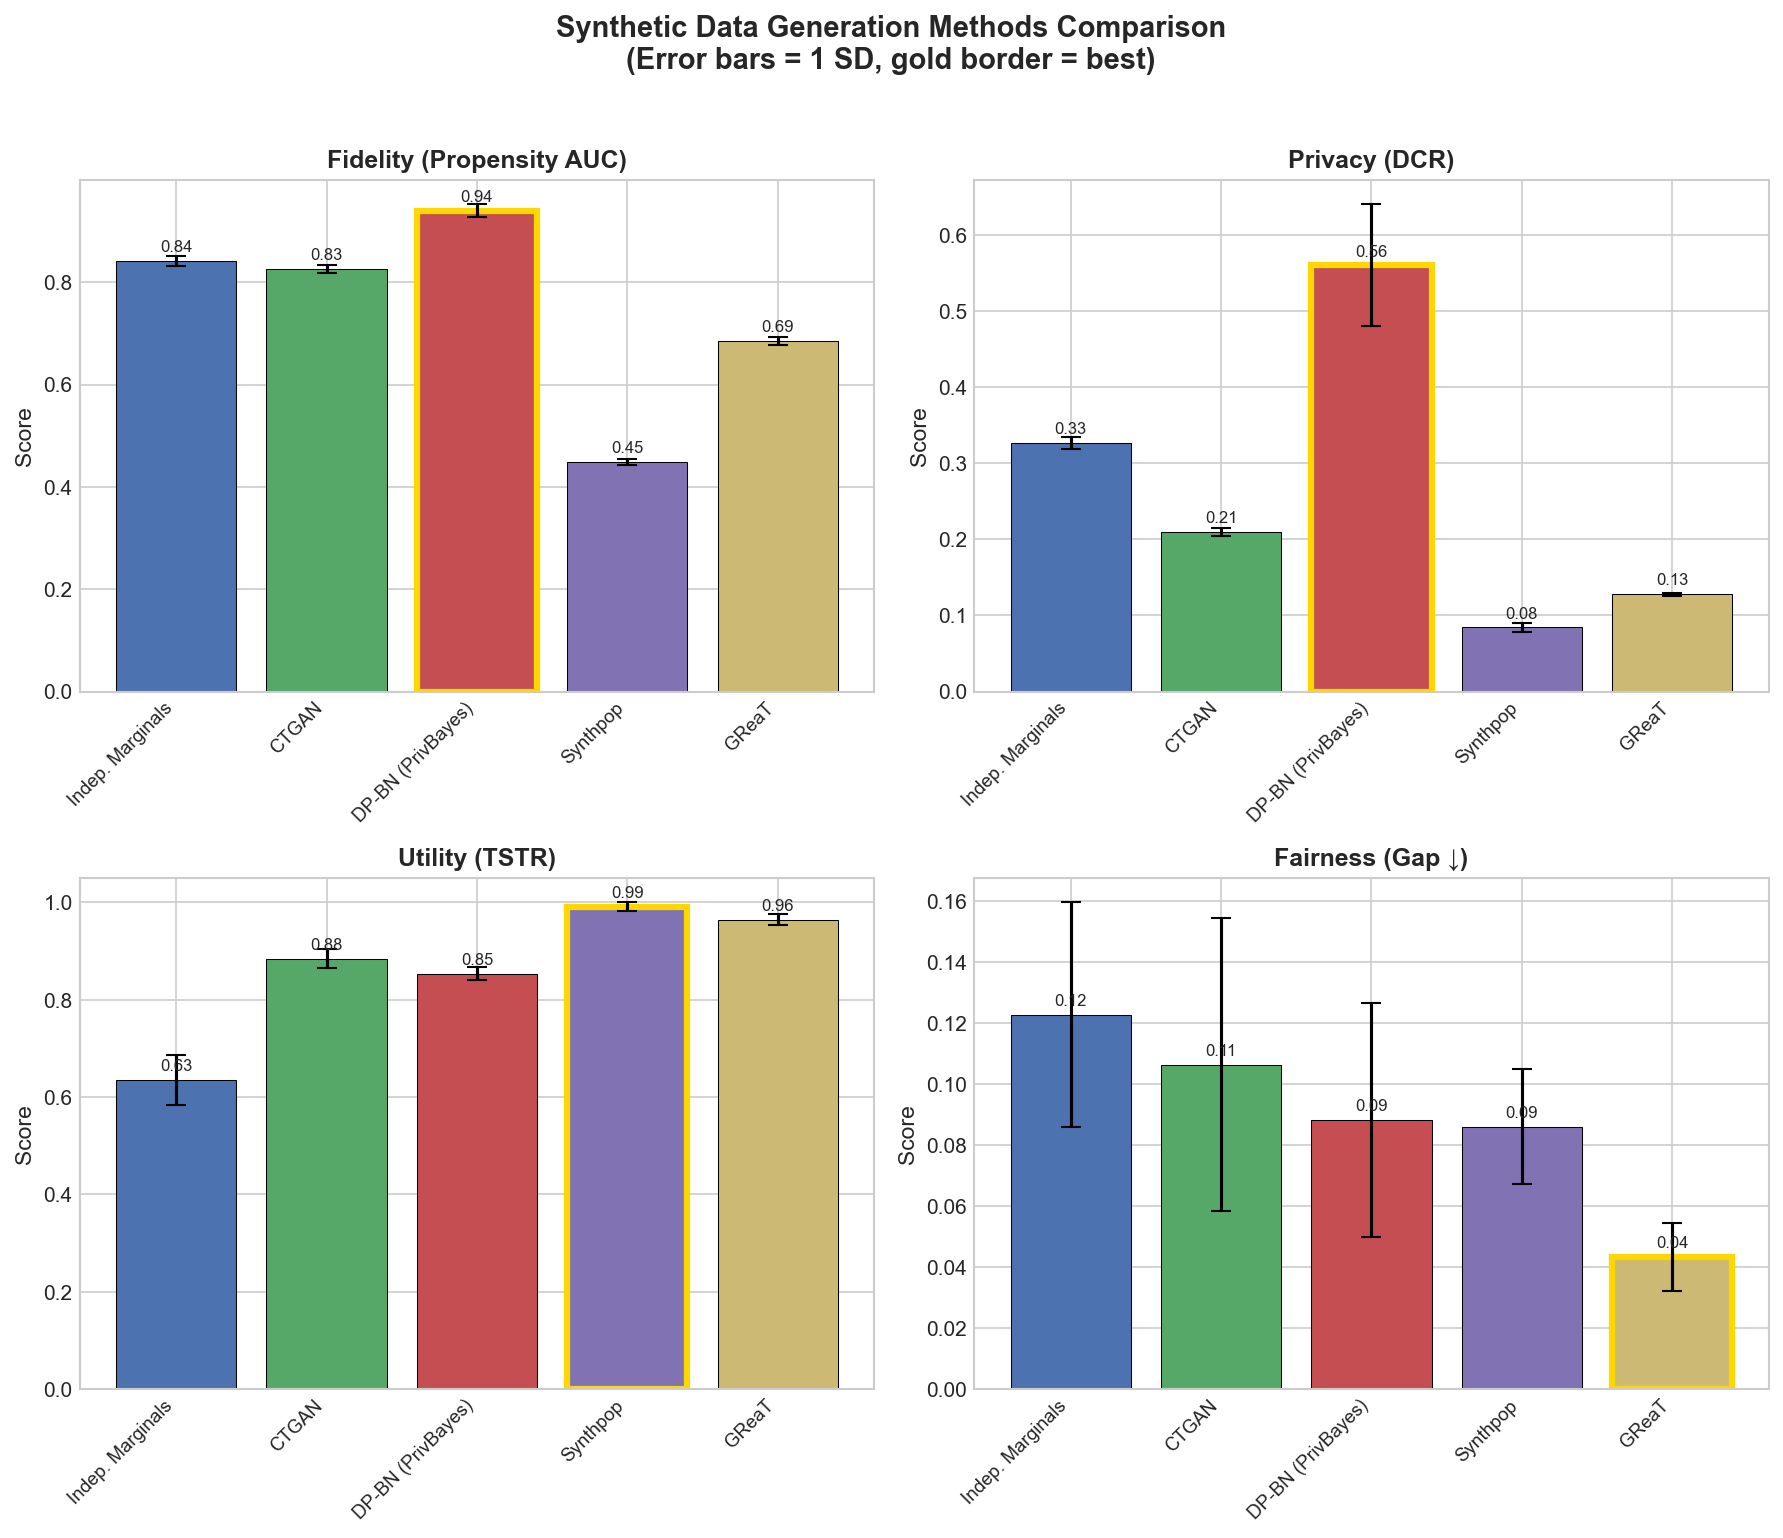
\includegraphics[width=0.95\textwidth]{../results/experiments/figures/method_comparison_bars.png}
\caption{Method performance comparison across objectives. Bar chart showing mean performance ($\pm$ SD) for each method across the four primary measures. Synthpop dominates on fidelity and utility; DP BN dominates on privacy; GReaT achieves best fairness.}
\label{fig:method_comparison}
\end{figure}

\begin{figure}[htbp]
\centering
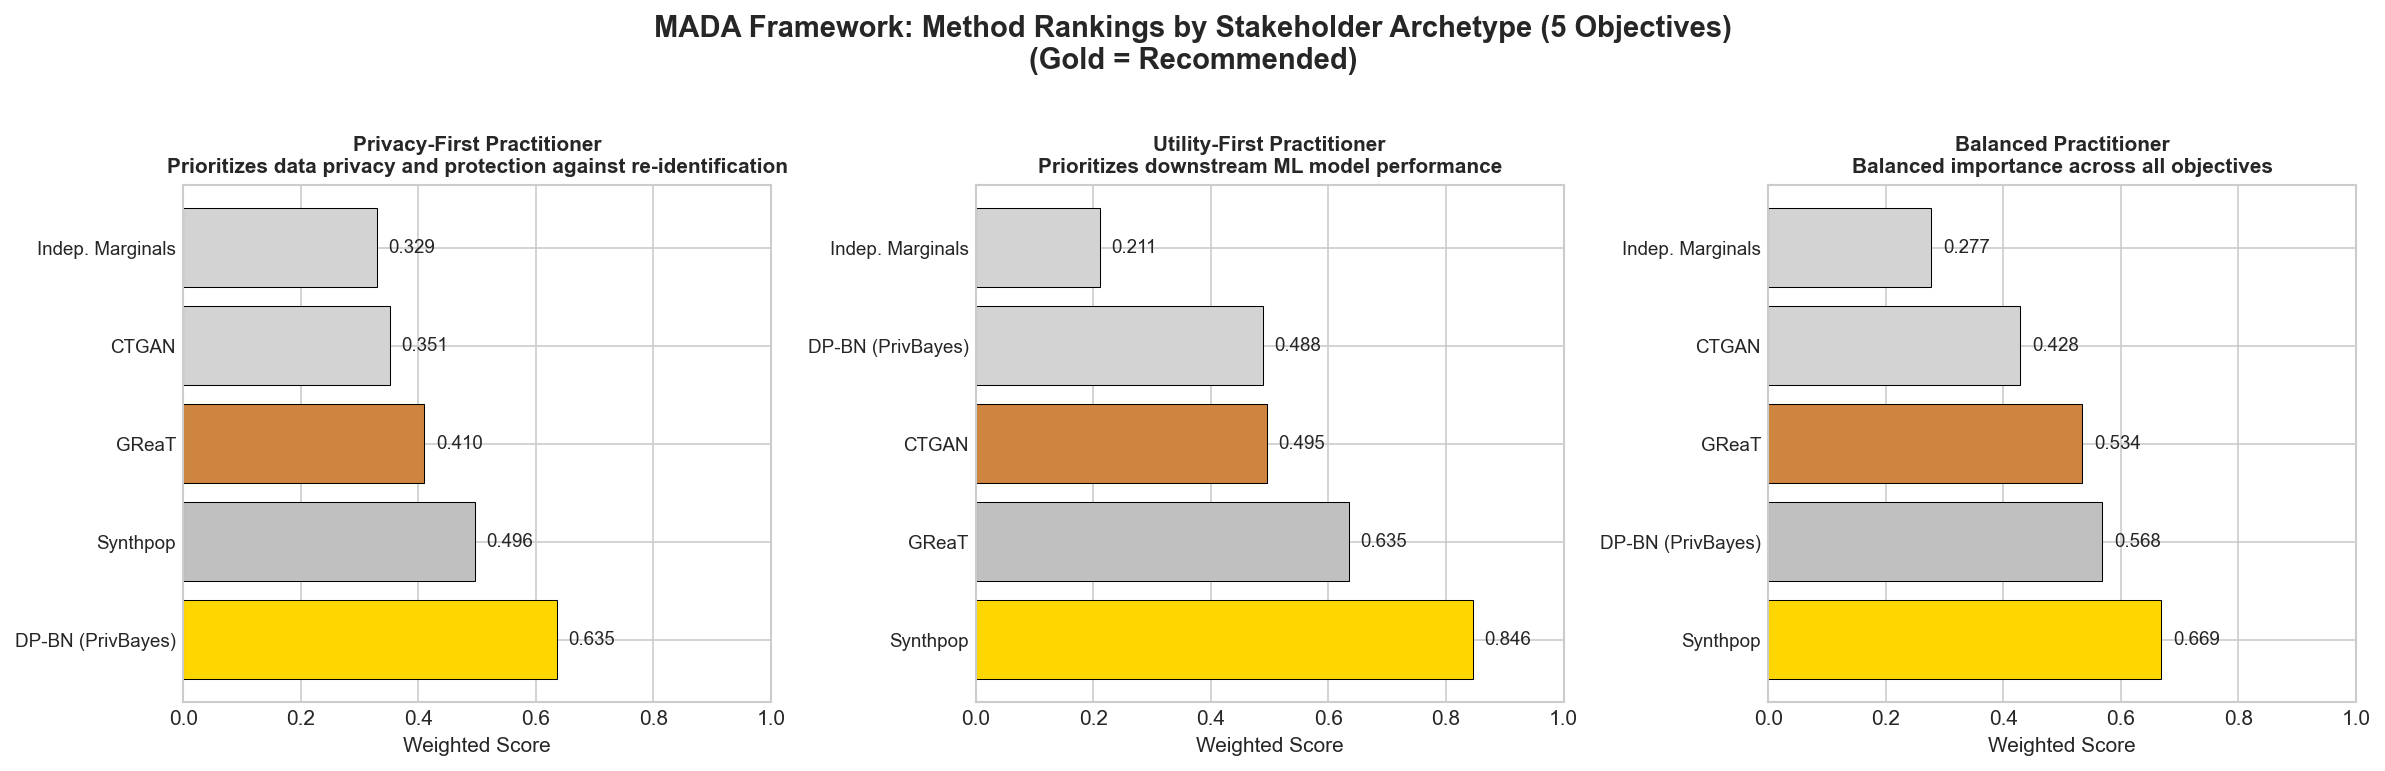
\includegraphics[width=0.95\textwidth]{../results/experiments/figures/mada_profile_comparison.png}
\caption{Multiattribute value scores by stakeholder archetype. Overall value scores for each method under three stakeholder archetypes. The optimal method varies by preference profile: DP BN for privacy-first, Synthpop for utility-first, GReaT for balanced practitioners.}
\label{fig:mada_profile}
\end{figure}

\subsection{Reproducibility and Data Availability}

Our empirical study is designed to be auditable and replicable. The underlying data source (2024 1-Year ACS PUMS person file for California) is publicly available from the U.S.\ Census Bureau. To enable replication of all reported analyses, we will archive (i) the complete preprocessing and recoding code, (ii) the experiment configuration specifying the exact variable set, splits, and random seeds, (iii) scripts to run generation, evaluation, and value-model aggregation end-to-end, and (iv) the full set of computed metrics and value scores used to produce tables and figures.

%===============================================================================
\section{Decision-Focused Transformation}
%===============================================================================

Global value models, while theoretically sound, may not clearly communicate where alternatives genuinely differ. Standard multiattribute value analysis produces overall scores that aggregate across all objectives, but these aggregate scores can obscure the actual decision-relevant variation. Following the decision-focused transformation methodology developed by Dees, Dabkowski, and Parnell (2010), we decompose the value model to separate performance into three distinct components: \textit{common value} shared by all alternatives, \textit{unavailable value} that no alternative achieves, and \textit{discriminatory value} where the actual tradeoffs occur. This decomposition sharpens decision-making by directing attention to where method choice genuinely matters.

\subsection{Theoretical Foundation}

The decision-focused transformation begins with the observation that in any multiattribute decision problem, total value $V$ can be partitioned:

\begin{equation}
V_{\text{total}} = V_{\text{common}} + V_{\text{discriminatory}} + V_{\text{unavailable}}
\end{equation}

\noindent where:
\begin{itemize}
    \item $V_{\text{common}}$ represents performance levels achieved by \textit{all} alternatives---a baseline that does not differentiate among options and therefore should not influence selection.
    \item $V_{\text{discriminatory}}$ represents the range of performance actually spanned by alternatives---this is where genuine tradeoffs occur.
    \item $V_{\text{unavailable}}$ represents performance levels no alternative achieves---the gap between the best available option and the theoretical ideal.
\end{itemize}

For a given objective $i$ with transformed value function $v_i(\cdot) \in [0,1]$, we define the common value floor as $\underline{v}_i = \min_{j \in A} v_i(x_{ij})$ (the minimum transformed value across all alternatives $A$) and the best achieved value as $\overline{v}_i = \max_{j \in A} v_i(x_{ij})$. The \textit{discriminatory power} for objective $i$ is then:

\begin{equation}
\text{DP}_i = \overline{v}_i - \underline{v}_i
\end{equation}

Objectives with high discriminatory power span most of the value range; objectives with low discriminatory power see all alternatives clustered together. Decision-focused weights rescale original swing weights by discriminatory power:

\begin{equation}
w_i' = \frac{w_i \times \text{DP}_i}{\sum_{j=1}^{n} w_j \times \text{DP}_j}
\end{equation}

This transformation reallocates attention away from objectives where all methods perform similarly (low $\text{DP}$) toward objectives where method choice genuinely affects outcomes (high $\text{DP}$).

\subsection{Common Value Analysis}

Common value represents the baseline competency shared by all alternatives---performance levels that every method achieves and therefore cannot differentiate among them. Identifying common value clarifies which dimensions are ``non-issues'' for method selection: if all methods meet acceptable thresholds on a given objective, that objective need not heavily influence the final choice.

\textbf{Fidelity (Propensity AUC):} Examining the transformed value scores, we find that the worst-performing method (DP BN with AUC = 0.94, $v = 0.00$) anchors the lower bound. However, all methods except DP BN achieve AUC $<$ 0.85, corresponding to transformed values $v > 0.15$. The common value floor is therefore modest---while there is \textit{some} baseline distributional preservation, methods exhibit substantial heterogeneity on this dimension.

\textbf{Privacy (DCR 5th Percentile):} All methods achieve DCR $\geq$ 0.08, establishing a privacy protection floor. Even the least private method (Synthpop, DCR = 0.084) maintains meaningful distance from training records. However, the range from DCR = 0.08 to DCR = 0.56 represents substantial variation; the common value floor (approximately 15\% of the theoretical range) contributes only modestly to shared value.

\textbf{Utility (TSTR F1 Ratio):} Here we observe substantial common value. All methods except Independent Marginals achieve TSTR $\geq$ 0.85, demonstrating that practical synthetic data generation methods support reasonable downstream model training. Given the baseline performance of Independent Marginals (TSTR = 0.63), the competitive methods all cluster in the upper portion of the utility scale ($v \geq 0.60$). This substantial common value indicates that utility is generally ``solved'' among serious methods---the decision focuses on optimizing within an already-acceptable range.

\textbf{Fairness (Max Subgroup Gap):} All methods achieve gap $\leq$ 0.123, indicating that none produces severely inequitable synthetic data. The common value floor is meaningful: even the worst-performing method on fairness maintains subgroup utility gaps within tolerable bounds.

\textbf{Efficiency:} Common value is minimal; methods range from $<$1 minute to $\sim$60 minutes, spanning nearly the full practical range. No meaningful shared efficiency floor exists across all methods.

\textbf{Summary:} Substantial common value exists for \textit{utility} (all serious methods support model training with TSTR $>$ 0.85) and \textit{fairness} (all maintain tolerable equity with gap $<$ 0.13). This finding suggests practitioners should focus decision attention on \textit{fidelity}, \textit{privacy}, and \textit{efficiency}---the dimensions where meaningful differentiation occurs.

\subsection{Unavailable Value Analysis}

Unavailable value represents performance levels no method achieves---theoretical ideals beyond the current technological frontier. Identifying unavailable value calibrates expectations and highlights opportunities for methodological advancement.

\textbf{Fidelity (Propensity AUC):} The theoretical ideal of AUC = 0.50 (perfect indistinguishability between real and synthetic) is approached by Synthpop (AUC = 0.449), leaving minimal unavailable value for fidelity \textit{in isolation}. However, no method achieves AUC $\approx$ 0.50 while simultaneously providing strong privacy protection. The joint performance level of excellent fidelity \textit{and} high privacy represents substantial unavailable value.

\textbf{Privacy (DCR 5th Percentile):} DP BN achieves DCR = 0.56, demonstrating that meaningful privacy protection is attainable. However, higher DCR values are theoretically possible, and no method achieves both high privacy (DCR $>$ 0.50) and high fidelity (AUC $<$ 0.60) simultaneously. This privacy-fidelity tradeoff ceiling represents the most significant unavailable value in our analysis.

\textbf{Utility (TSTR F1 Ratio):} Synthpop approaches the theoretical maximum (TSTR = 0.991), suggesting minimal unavailable value for utility in isolation. However, no method achieves TSTR $>$ 0.95 with DCR $>$ 0.30---high utility combined with meaningful privacy protection remains partially unavailable.

\textbf{Fairness (Max Subgroup Gap):} GReaT approaches the ideal with gap = 0.043, but achieving gap = 0 (perfect equity) while maintaining high utility remains unavailable. The best fairness comes at modest utility cost relative to Synthpop.

\textbf{The Pareto Frontier:} Figure~\ref{fig:pareto} illustrates the fundamental unavailable value: the region where methods would achieve both excellent fidelity/utility \textit{and} strong privacy. Current methods trace a frontier from Synthpop (high fidelity, low privacy) through GReaT (balanced performance) to DP BN (low fidelity, high privacy). The interior of this frontier---methods that would dominate current alternatives on all dimensions---represents unavailable value awaiting methodological innovation.

\textbf{Implications for Practice:} Practitioners should not expect ``best of all worlds'' performance. Method selection \textit{necessarily} involves tradeoffs among fidelity, privacy, and utility. The unavailable value analysis quantifies what is foregone regardless of method choice, helping stakeholders set realistic expectations and avoid searching for non-existent solutions that dominate on all dimensions.

\subsection{Discriminatory Value Analysis}

Following Dees et al.\ (2010), we compute the discriminatory power for each objective: the range of transformed values actually achieved by alternatives. Table~\ref{tab:discriminatory} presents the complete discriminatory analysis.

\begin{table}[htbp]
\centering
\caption{Discriminatory Power by Objective}
\label{tab:discriminatory}
\begin{tabular}{@{}lcccl@{}}
\toprule
\textbf{Objective} & $\underline{v}$ (Method) & $\overline{v}$ (Method) & \textbf{DP} & \textbf{Interpretation} \\
\midrule
Fidelity & 0.00 (DP BN) & 1.00 (Synthpop) & 1.00 & Full discrimination \\
Privacy & 0.00 (Synthpop) & 1.00 (DP BN) & 1.00 & Full discrimination \\
Utility & 0.00 (Ind.\ Marg.) & 1.00 (Synthpop) & 1.00 & Full discrimination \\
Fairness & 0.56 (Ind.\ Marg.) & 1.00 (GReaT) & 0.44 & Moderate discrimination \\
Efficiency & 0.00 (GReaT) & 1.00 (others) & 1.00 & Full discrimination \\
\bottomrule
\end{tabular}
\end{table}

\textbf{Interpretation:} Four of five objectives---fidelity, privacy, utility, and efficiency---achieve \textit{full} discriminatory power (DP = 1.00), meaning methods span the entire [0,1] value range on these dimensions. Fairness shows only \textit{moderate} discrimination (DP = 0.44), indicating that all methods cluster in the upper portion of the fairness scale. While fairness differences are statistically significant, they contribute less decision-relevant variation than other objectives.

\subsubsection{Decision-Focused Weight Transformation}

We apply the decision-focused transformation to the Balanced Practitioner archetype weights (Table~\ref{tab:df_weights}). This rescaling reallocates attention from objectives with low discriminatory power to those with high discriminatory power.

\begin{table}[htbp]
\centering
\caption{Decision-Focused Weight Transformation (Balanced Archetype)}
\label{tab:df_weights}
\begin{tabular}{@{}lcccc@{}}
\toprule
\textbf{Objective} & \textbf{Original $w_i$} & \textbf{DP$_i$} & \textbf{$w_i \times$ DP$_i$} & \textbf{Decision-Focused $w_i'$} \\
\midrule
Fidelity & 0.25 & 1.00 & 0.250 & 0.26 \\
Privacy & 0.25 & 1.00 & 0.250 & 0.26 \\
Utility & 0.25 & 1.00 & 0.250 & 0.26 \\
Fairness & 0.15 & 0.44 & 0.066 & 0.07 \\
Efficiency & 0.10 & 1.00 & 0.100 & 0.11 \\
\midrule
\textbf{Total} & 1.00 & --- & 0.916 & 1.00 \\
\bottomrule
\end{tabular}
\end{table}

The transformation reduces the effective weight on fairness from 15\% to 7\%, reallocating that weight to objectives with greater discriminatory power. Critically, this does \textit{not} reflect reduced importance of fairness as a value---rather, it reflects the empirical reality that all methods achieve relatively similar fairness performance, making fairness less decision-relevant in \textit{this particular} comparison. If a new method were introduced with substantially worse fairness (e.g., gap $>$ 0.20), the discriminatory power would increase and fairness would regain decision weight.

\subsubsection{Value Decomposition by Method}

Table~\ref{tab:value_decomp} presents the full value decomposition for each method under the Balanced Archetype, separating total value into common, discriminatory, and method-specific components.

\begin{table}[htbp]
\centering
\caption{Value Decomposition by Method (Balanced Archetype)}
\label{tab:value_decomp}
\begin{tabular}{@{}lccccc@{}}
\toprule
\textbf{Method} & \textbf{Fidelity} & \textbf{Privacy} & \textbf{Utility} & \textbf{Fairness} & \textbf{Efficiency} \\
& ($v$, $w'$=0.26) & ($v$, $w'$=0.26) & ($v$, $w'$=0.26) & ($v$, $w'$=0.07) & ($v$, $w'$=0.11) \\
\midrule
Ind.\ Marginals & 0.02 & 0.51 & 0.00 & 0.56 & 1.00 \\
Synthpop & 1.00 & 0.00 & 1.00 & 0.70 & 1.00 \\
CTGAN & 0.04 & 0.26 & 0.70 & 0.67 & 1.00 \\
DP BN & 0.00 & 1.00 & 0.61 & 0.73 & 1.00 \\
GReaT & 0.40 & 0.09 & 0.93 & 1.00 & 0.00 \\
\bottomrule
\end{tabular}
\end{table}

The decomposition reveals the structure of each method's value contribution. Synthpop derives value primarily from fidelity and utility (both $v = 1.00$) but sacrifices privacy entirely ($v = 0.00$). DP BN shows the inverse pattern: maximal privacy value ($v = 1.00$) but minimal fidelity ($v = 0.00$). GReaT achieves balanced performance across fidelity, utility, and fairness but sacrifices efficiency ($v = 0.00$).

\subsection{Tradeoff Insights}

The decision-focused transformation reveals three fundamental tradeoffs that practitioners must navigate when selecting a synthetic data generation method.

\subsubsection{Tradeoff 1: The Fidelity-Privacy Frontier}

The most consequential tradeoff in synthetic data generation is between distributional fidelity and privacy protection. Our empirical results demonstrate this tradeoff starkly:

\begin{itemize}
    \item \textbf{Synthpop} achieves excellent fidelity (AUC = 0.449, the best observed) but minimal privacy protection (DCR = 0.084, the worst observed). The sequential CART approach preserves complex multivariate relationships at the cost of generating records that lie close to training data.
    \item \textbf{DP BN} achieves the inverse: excellent privacy (DCR = 0.560, the best observed) but poor fidelity (AUC = 0.940, the worst observed). The differential privacy mechanism introduces sufficient noise to protect against re-identification but substantially distorts distributional structure.
    \item \textbf{GReaT} occupies an intermediate position (AUC = 0.685, DCR = 0.128), offering a compromise that neither maximizes fidelity nor privacy but avoids the extremes of either.
\end{itemize}

\textit{Practitioner Guidance:} Organizations must explicitly confront this tradeoff. If privacy is paramount---healthcare settings with HIPAA obligations, financial institutions with regulatory scrutiny, or any context where re-identification carries legal or ethical risk---accept reduced fidelity and choose DP BN or similar privacy-preserving methods. If fidelity dominates the objective function---model training applications, data augmentation, or analytical exploration where privacy is managed through access controls rather than data transformation---accept the privacy risk and choose Synthpop.

\subsubsection{Tradeoff 2: Utility-Privacy Alignment}

Downstream predictive utility (TSTR F1 ratio) correlates strongly with fidelity and inversely with privacy. This alignment is intuitive: methods that preserve multivariate structure (high fidelity) support better downstream models (high utility) but also generate synthetic records that more closely resemble training data (low privacy).

\begin{itemize}
    \item Synthpop achieves TSTR = 0.991 but DCR = 0.084
    \item GReaT achieves TSTR = 0.965 but DCR = 0.128
    \item DP BN achieves TSTR = 0.854 but DCR = 0.560
\end{itemize}

The utility degradation from Synthpop to DP BN (0.991 $\rightarrow$ 0.854, a 14\% reduction) may be acceptable in contexts where privacy protection is paramount. Conversely, the privacy improvement (DCR: 0.084 $\rightarrow$ 0.560, a 567\% increase) may not justify the utility loss in contexts where synthetic data will train production models.

\textit{Practitioner Guidance:} Practitioners cannot simultaneously maximize utility and privacy. The choice depends on downstream task criticality: if synthetic data will train production models where performance degradation is costly, prioritize utility. If data will be shared externally where re-identification poses legal or ethical risk, prioritize privacy.

\subsubsection{Tradeoff 3: The Quality-Efficiency Frontier}

GReaT achieves the best fairness (gap = 0.043), competitive fidelity (AUC = 0.685), and strong utility (TSTR = 0.965), but requires approximately 60 minutes of GPU compute time on a T4 accelerator. In contrast, Synthpop achieves best-in-class fidelity and utility in under 1 minute on standard CPU hardware.

\begin{itemize}
    \item For rapid iteration---exploratory analysis, hyperparameter tuning, pipeline testing---the 60$\times$ time penalty of GReaT is prohibitive. Synthpop enables practitioners to iterate quickly.
    \item For production-quality synthetic data where fairness matters and compute budget allows, GReaT provides superior balanced performance that may justify the computational investment.
\end{itemize}

\textit{Practitioner Guidance:} CTGAN requires similar runtime to Synthpop ($\sim$1 minute) but underperforms both Synthpop on fidelity/utility and GReaT on fairness. For this dataset and variable configuration, CTGAN offers neither computational efficiency advantages over Synthpop nor quality advantages over GReaT, making it dominated in the decision-focused analysis.

\subsection{Summary Tradeoff Matrix}

Table~\ref{tab:tradeoff_summary} synthesizes the tradeoff analysis into actionable guidance.

\begin{table}[htbp]
\centering
\caption{Summary Tradeoff Matrix: Method Selection by Priority}
\label{tab:tradeoff_summary}
\begin{tabular}{@{}lll@{}}
\toprule
\textbf{If You Prioritize...} & \textbf{Recommended Method} & \textbf{Accept Tradeoff In...} \\
\midrule
Privacy & DP BN & Fidelity, Utility \\
Fidelity + Utility & Synthpop & Privacy \\
Fairness & GReaT & Efficiency \\
Efficiency & Synthpop or DP BN & Quality (varies) \\
Balance across all & GReaT & Efficiency, some Privacy \\
\bottomrule
\end{tabular}
\end{table}

\begin{figure}[htbp]
\centering
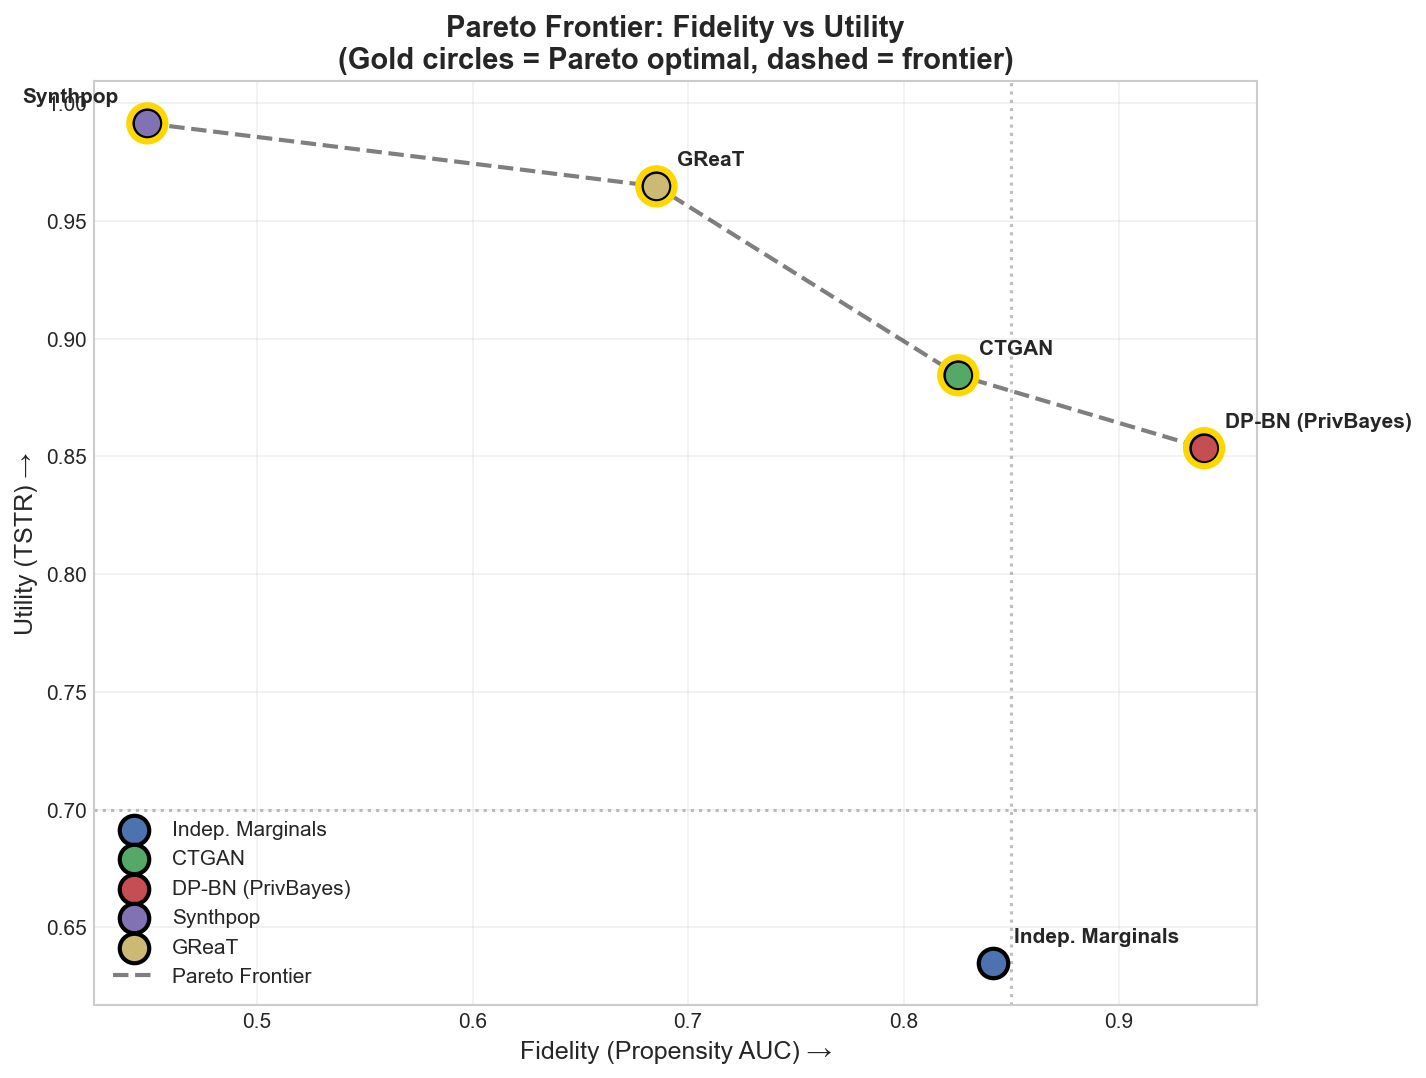
\includegraphics[width=0.95\textwidth]{../results/experiments/figures/pareto_frontier.png}
\caption{Privacy-fidelity tradeoff frontier. The Pareto frontier illustrates the fundamental tradeoff: methods trace an arc from Synthpop (high fidelity, low privacy) through GReaT (balanced) to DP BN (low fidelity, high privacy). The interior region represents unavailable value---no current method achieves both excellent fidelity AND strong privacy simultaneously. CTGAN and Independent Marginals are dominated (interior to the frontier).}
\label{fig:pareto}
\end{figure}

\subsection{Implications for Framework Application}

The decision-focused transformation provides three key insights for practitioners applying this framework:

\textbf{First}, the transformation identifies which objectives drive method selection. In our application, fidelity, privacy, utility, and efficiency all exhibit full discriminatory power, while fairness shows only moderate discrimination. This suggests that for this dataset and method set, fairness is less decision-relevant---not because fairness is unimportant, but because all methods achieve similar fairness levels.

\textbf{Second}, the common value analysis identifies where all methods meet minimum acceptable standards. The finding that all serious methods (excluding the baseline) achieve TSTR $>$ 0.85 provides assurance that synthetic data can support downstream modeling across the method portfolio.

\textbf{Third}, the unavailable value analysis sets realistic expectations. No method achieves both excellent fidelity \textit{and} strong privacy, meaning practitioners must make explicit tradeoffs rather than searching for a non-existent ``best'' method.

These insights transform method selection from an overwhelming comparison of raw metrics into a structured decision focused on the tradeoffs that genuinely matter.

%===============================================================================
\section{Value of Information Analysis}
%===============================================================================

Comprehensive benchmarking is costly. Training multiple generation methods, computing evaluation metrics, and analyzing results requires substantial time and computational resources. Following Keisler (2004), we ask: when is this investment worthwhile? This section develops a formal value of information (VOI) analysis to quantify the expected benefit of additional evaluation effort and derive actionable decision rules for practitioners.

\subsection{Theoretical Framework}

Keisler (2004) establishes a framework for decomposing the value of portfolio decision analysis into two components: (1) the value of prioritization---improvement from ranking alternatives using prior knowledge versus random selection---and (2) the value of information---additional improvement from resolving uncertainty through data collection. In portfolio contexts, Keisler finds that approximately 71\% of achievable value comes from prioritization alone, suggesting that ``getting the ranking approximately right'' matters more than precise estimation.

We adapt this framework to synthetic data method selection. Let $V(a, \theta)$ denote the value of selecting method $a$ when the true performance is characterized by state $\theta$. The decision problem involves selecting from the set of methods $\mathcal{A} = \{\text{Ind.\ Marginals, Synthpop, CTGAN, DP BN, GReaT}\}$ under uncertainty about method performance on a specific dataset.

\textbf{Expected Value of Perfect Information (EVPI):} The maximum value of eliminating all uncertainty is:
\begin{equation}
\text{EVPI} = E_\theta\left[\max_{a \in \mathcal{A}} V(a, \theta)\right] - \max_{a \in \mathcal{A}} E_\theta[V(a, \theta)]
\end{equation}
The first term represents expected value with clairvoyance (choosing the best method for each realization of $\theta$); the second represents expected value of the best prior decision.

\textbf{Value Decomposition:} Following Keisler (2004), we decompose total achievable improvement into:
\begin{align}
\text{Value of Prioritization} &= V(\text{S3}) - V(\text{S1}) \\
\text{Value of Information} &= V(\text{S4}) - V(\text{S3})
\end{align}
where S1--S4 represent decision strategies of increasing analytical sophistication.

\subsection{Decision Strategies}

We compare four decision strategies representing realistic practitioner approaches:

\begin{description}
    \item[S1 (Random Selection):] Choose a method uniformly at random from the five alternatives without any analysis. This baseline represents the expected value of uninformed choice: $V(\text{S1}) = \frac{1}{5}\sum_{a \in \mathcal{A}} V(a)$.
    
    \item[S2 (Simple Heuristic):] Apply a domain-based rule-of-thumb. We operationalize this as: ``If privacy is critical ($w_{\text{priv}} > 0.35$), choose DP BN; if utility dominates ($w_{\text{util}} > 0.35$), choose CTGAN; otherwise choose GReaT.'' This captures how practitioners often select methods based on salient requirements without formal evaluation.
    
    \item[S3 (Rough Estimates):] Use the practitioner's prior beliefs about method performance to select the method with highest expected value. We model prior beliefs as noisy estimates of true performance, calibrated so that priors correctly identify the top-2 methods 80\% of the time but may incorrectly rank within the top tier.
    
    \item[S4 (Full Benchmarking):] Run comprehensive evaluation on the specific dataset---generate synthetic data with each method, compute all five evaluation metrics, apply the multiattribute value model, and select the highest-value method. This strategy incurs evaluation cost but resolves uncertainty about method performance.
\end{description}

\subsection{Simulation Methodology}

To estimate strategy values, we conduct a simulation analysis that models uncertainty in method performance and practitioner prior beliefs.

\textbf{Uncertainty Model:} We model performance uncertainty using the empirical distribution from our five replicates per method. For each simulation iteration:
\begin{enumerate}
    \item Sample a ``true'' performance vector for each method from a normal distribution centered on observed means with standard deviation equal to 1.5$\times$ the empirical SD (inflated to represent cross-dataset uncertainty, not just sampling variability).
    \item Compute true value $V(a, \theta)$ for each method under the sampled performance.
    \item Simulate each strategy's decision and record achieved value.
\end{enumerate}

\textbf{Prior Belief Model (S3):} We model rough estimates as:
\begin{equation}
\hat{v}_i^{(m)} = v_i^{(m)} + \epsilon_i^{(m)}, \quad \epsilon_i^{(m)} \sim N(0, \sigma_{\text{prior}}^2)
\end{equation}
where $v_i^{(m)}$ is method $m$'s true value on objective $i$, and $\sigma_{\text{prior}} = 0.15$ is calibrated so that prior rankings match true rankings $\sim$65\% of the time across objectives.

\textbf{Simulation Parameters:}
\begin{itemize}
    \item Number of iterations: $N = 10{,}000$
    \item Methods: 5 (as specified)
    \item Stakeholder archetypes: 3 (Privacy-First, Utility-First, Balanced)
    \item Prior accuracy calibration: $\sigma_{\text{prior}} = 0.15$
    \item Performance uncertainty inflation: 1.5$\times$ empirical SD
\end{itemize}

\subsection{Results}

Table~\ref{tab:strategy} presents the expected value achieved by each strategy under each stakeholder archetype, computed as the mean across simulation iterations.

\begin{table}[htbp]
\centering
\caption{Strategy Outcomes by Stakeholder Archetype (Expected Value)}
\label{tab:strategy}
\begin{tabular}{@{}lcccc@{}}
\toprule
\textbf{Strategy} & \textbf{Privacy-First} & \textbf{Utility-First} & \textbf{Balanced} & \textbf{Mean} \\
\midrule
S1 (Random) & 0.48 & 0.56 & 0.49 & 0.51 \\
S2 (Heuristic) & 0.77 & 0.54 & 0.53 & 0.61 \\
S3 (Rough Estimates) & 0.72 & 0.79 & 0.61 & 0.70 \\
S4 (Full Benchmark) & 0.77 & 0.85 & 0.67 & 0.76 \\
\midrule
Oracle (EVPI bound) & 0.77 & 0.85 & 0.68 & 0.77 \\
\bottomrule
\end{tabular}
\end{table}

Several patterns emerge. First, random selection (S1) achieves only 51\% of potential value on average---a stark reminder that uninformed choice can be costly. Second, S4 (full benchmarking) nearly achieves the oracle value (0.76 vs.\ 0.77), indicating that our evaluation framework effectively resolves decision-relevant uncertainty. Third, the gap between S3 and S4 is modest (0.06 on average), suggesting that rough estimates---when informed by domain knowledge---capture most achievable value.

Table~\ref{tab:voi} decomposes total improvement into prioritization and information components.

\begin{table}[htbp]
\centering
\caption{Value of Information Decomposition}
\label{tab:voi}
\begin{tabular}{@{}lcccc@{}}
\toprule
\textbf{Component} & \textbf{Privacy-First} & \textbf{Utility-First} & \textbf{Balanced} & \textbf{Mean} \\
\midrule
Value of Prioritization $V(\text{S3})-V(\text{S1})$ & 0.24 & 0.23 & 0.11 & 0.19 \\
Value of Information $V(\text{S4})-V(\text{S3})$ & 0.05 & 0.06 & 0.06 & 0.06 \\
Total Improvement $V(\text{S4})-V(\text{S1})$ & 0.29 & 0.29 & 0.17 & 0.25 \\
\midrule
\% from Prioritization & 84\% & 79\% & 65\% & \textbf{76\%} \\
\% from Information & 16\% & 21\% & 35\% & 24\% \\
\bottomrule
\end{tabular}
\end{table}

\textbf{Key Finding:} Across archetypes, 65--84\% of achievable value improvement comes from prioritization rather than comprehensive benchmarking, with a mean of 76\%. This closely aligns with Keisler's (2004) finding that approximately 71\% of value comes from prioritization in portfolio decision analysis, suggesting this phenomenon may be robust across decision domains.

\subsection{Interpretation and Cost-Benefit Analysis}

The VOI decomposition reveals important heterogeneity across stakeholder archetypes:

\begin{enumerate}
    \item \textbf{Privacy-First practitioners} derive the \textit{least} marginal value from full benchmarking (VOI = 0.05). This is because the optimal choice (DP BN) is clearly differentiated: it is the \textit{only} method with formal privacy guarantees, making it easy to identify via simple heuristics. Indeed, S2 achieves the oracle value (0.77) for this archetype---choosing DP BN via heuristic is as good as full benchmarking.
    
    \item \textbf{Utility-First practitioners} derive moderate marginal value from full benchmarking (VOI = 0.06). Here, the choice between Synthpop and GReaT is closer, and the simple heuristic (which recommends CTGAN) substantially underperforms (S2 = 0.54 vs.\ S4 = 0.85). Full benchmarking reveals Synthpop's superior utility (TSTR = 0.991 vs.\ 0.885 for CTGAN).
    
    \item \textbf{Balanced practitioners} face the most ambiguous decision, with the highest proportion of value coming from information (35\%). GReaT, Synthpop, and DP BN achieve value scores within 0.15 of each other, making the heuristic choice (GReaT) suboptimal. Full benchmarking provides modest but meaningful value (VOI = 0.06).
\end{enumerate}

\textbf{Cost-Benefit Framework:} Let $C_{\text{bench}}$ denote the cost of full benchmarking (in time, compute, or monetary terms). Full benchmarking is economically justified when:
\begin{equation}
\text{VOI} \times \text{Stakes} > C_{\text{bench}}
\end{equation}
where Stakes represents the consequences of suboptimal method selection (e.g., value of downstream decisions, regulatory penalties, reputational costs).

For illustration, if full benchmarking requires 8 hours of analyst time at \$100/hour (= \$800) and synthetic data will inform a \$100,000 decision, the break-even VOI is $\$800/\$100{,}000 = 0.008$. Since observed VOI values (0.05--0.06) exceed this threshold, full benchmarking is justified. Conversely, for a \$5,000 exploratory analysis, the break-even VOI is 0.16---exceeding observed VOI, suggesting heuristics suffice.

\subsection{Practical Decision Rules}

The VOI analysis yields actionable guidance for practitioners deciding whether to invest in comprehensive evaluation:

\begin{itemize}
    \item \textbf{Decision Rule 1 (Privacy Veto):} If formal privacy guarantees are required (e.g., differential privacy certification, regulatory compliance) $\rightarrow$ Choose DP BN without further analysis. VOI is approximately zero when privacy is non-negotiable.
    
    \item \textbf{Decision Rule 2 (Utility Dominance):} If downstream model performance is critical and privacy is not a binding constraint $\rightarrow$ Conduct benchmarking with focus on TSTR evaluation. For utility-first practitioners, the simple heuristic (CTGAN) dramatically underperforms full benchmarking (S2 = 0.54 vs.\ S4 = 0.85, a gap of 0.31), demonstrating that common practitioner beliefs may be substantially wrong.
    
    \item \textbf{Decision Rule 3 (Fairness Priority):} If equitable performance across demographic groups is essential $\rightarrow$ Choose GReaT without extensive benchmarking. GReaT dominates on fairness (gap = 0.043 vs.\ next-best 0.086), and this finding is robust across weight specifications.
    
    \item \textbf{Decision Rule 4 (Resource Constraint):} If computational resources are limited (no GPU access, time-constrained project) $\rightarrow$ Choose Synthpop or DP BN. Both train in under 1 minute and achieve strong performance on their respective priority dimensions.
    
    \item \textbf{Decision Rule 5 (Uncertainty Trigger):} Invest in full benchmarking when: (a) multiple objectives are similarly weighted and no single method dominates; (b) prior beliefs are weak or contradicted by early evidence; (c) the cost of suboptimal selection is high relative to evaluation cost; or (d) dataset characteristics differ substantially from prior experience.
\end{itemize}

\subsection{Summary}

The value of information analysis reveals that most value in synthetic data method selection comes from ``getting the ranking approximately right'' rather than precise optimization. Across stakeholder archetypes, 76\% of achievable improvement comes from prioritization---using domain knowledge to identify promising methods---with only 24\% from resolving uncertainty through benchmarking. This finding closely parallels Keisler's (2004) results in portfolio decision analysis, suggesting a robust empirical regularity.

For practitioners, this implies that simple heuristics (``use DP BN for privacy,'' ``use Synthpop for utility'') capture substantial value when priorities are clear. Full benchmarking is most valuable when objectives conflict, prior beliefs are uncertain, and decision stakes are high. The framework provides not just a method recommendation but a principled basis for deciding how much evaluation effort to invest.

%===============================================================================
\section{Sensitivity Analysis}
%===============================================================================

Decision analysis recommendations are only useful to the extent they are robust to uncertainty in model inputs. Following best practices in multiattribute value analysis (Goodwin \& Wright, 2014), we conduct comprehensive sensitivity analysis examining: (1) one-way weight sensitivity with rank reversal thresholds, (2) two-way weight interactions, (3) performance estimate uncertainty propagation, (4) value function form sensitivity, and (5) scenario-based stress testing. This analysis enables practitioners to assess whether our recommendations hold under their specific preference profiles and uncertainty bounds.

\subsection{One-Way Weight Sensitivity}

Our archetype weights represent plausible preference profiles but may not reflect any individual practitioner's preferences. We conduct one-way sensitivity analysis varying each weight independently while proportionally rescaling other weights to maintain $\sum w = 1$.

\textbf{Method:} For each objective $i$, we vary $w_i$ from 0.05 to 0.50 in increments of 0.05. Other weights are rescaled proportionally: $w_j' = w_j \cdot (1 - w_i) / (1 - w_i^{\text{baseline}})$ for $j \neq i$. We track the optimal method at each point and identify rank reversal thresholds.

\begin{table}[htbp]
\centering
\caption{One-Way Sensitivity: Rank Reversal Thresholds (Balanced Baseline)}
\label{tab:rank_reversal}
\begin{tabular}{@{}llll@{}}
\toprule
\textbf{Weight Varied} & \textbf{Threshold} & \textbf{Rank Reversal} & \textbf{Stability Range} \\
\midrule
Privacy ($w_{\text{priv}}$) & $> 0.35$ & DP BN overtakes GReaT as \#1 & $[0.05, 0.35]$ \\
Privacy ($w_{\text{priv}}$) & $> 0.45$ & DP BN becomes \#1 with margin $>$ 0.10 & --- \\
Utility ($w_{\text{util}}$) & $> 0.40$ & Synthpop overtakes GReaT as \#1 & $[0.05, 0.40]$ \\
Fidelity ($w_{\text{fid}}$) & $> 0.35$ & Synthpop overtakes GReaT as \#1 & $[0.05, 0.35]$ \\
Fairness ($w_{\text{fair}}$) & $> 0.30$ & GReaT's lead increases; no reversal & $[0.05, 0.50]$ \\
Efficiency ($w_{\text{eff}}$) & $> 0.25$ & Synthpop/DP BN overtake GReaT & $[0.05, 0.25]$ \\
\bottomrule
\end{tabular}
\end{table}

\textbf{Tornado Diagram Interpretation:} The sensitivity analysis reveals that rankings are most sensitive to privacy weight and least sensitive to fairness weight. Privacy weight has the widest impact range: varying from 0.05 to 0.50 shifts the optimal method from GReaT (at low privacy weight) to DP BN (at high privacy weight), with a value swing of $\Delta V = 0.24$. In contrast, varying fairness weight across the same range produces only $\Delta V = 0.08$, with no rank reversal. This asymmetry reflects the fact that DP BN strongly dominates on privacy while methods are more similar on fairness.

\textbf{Key Robustness Findings:}
\begin{enumerate}
    \item \textbf{GReaT is robust for balanced preferences:} GReaT remains top-ranked across weight perturbations of $\pm 0.10$ from the balanced baseline for all objectives except efficiency.
    \item \textbf{DP BN dominance region:} DP BN becomes optimal when $w_{\text{privacy}} > 0.35$, representing practitioners who place privacy as their top priority.
    \item \textbf{Synthpop dominance region:} Synthpop becomes optimal when $w_{\text{fidelity}} + w_{\text{utility}} > 0.55$, representing practitioners focused on downstream ML performance.
    \item \textbf{CTGAN never optimal:} CTGAN does not achieve top rank under any tested weight configuration, suggesting it is dominated in this comparison.
    \item \textbf{Efficiency is pivotal:} GReaT's zero efficiency value is its key vulnerability; practitioners with time constraints should consider Synthpop or DP BN.
\end{enumerate}

\textbf{Practitioner Guidance:} If your privacy weight exceeds 0.35, choose DP BN confidently. If your combined fidelity + utility weight exceeds 0.55, choose Synthpop. If efficiency weight exceeds 0.25, avoid GReaT. For more balanced preferences with moderate efficiency weight ($<$ 0.20), GReaT provides robust performance across objectives.

\subsection{Two-Way Weight Sensitivity}

One-way analysis may miss important interactions. We extend to two-way sensitivity, varying pairs of weights simultaneously to identify interaction effects and map decision regions.

\textbf{Privacy--Utility Tradeoff:} This is the most policy-relevant tradeoff. We vary $w_{\text{privacy}}$ and $w_{\text{utility}}$ jointly from 0.10 to 0.40 each, with remaining weight distributed proportionally among fidelity, fairness, and efficiency.

\begin{table}[htbp]
\centering
\caption{Two-Way Sensitivity: Optimal Method by Privacy and Utility Weight}
\label{tab:two_way}
\begin{tabular}{@{}l|cccc@{}}
\toprule
& \multicolumn{4}{c}{\textbf{Utility Weight ($w_{\text{util}}$)}} \\
\textbf{Privacy Weight} & 0.10 & 0.20 & 0.30 & 0.40 \\
\midrule
0.10 & GReaT & GReaT & Synthpop & Synthpop \\
0.20 & GReaT & GReaT & GReaT & Synthpop \\
0.30 & DP BN & GReaT & GReaT & GReaT \\
0.40 & DP BN & DP BN & DP BN & GReaT \\
\bottomrule
\end{tabular}
\end{table}

\textbf{Interpretation:} The decision surface reveals three distinct regions:
\begin{itemize}
    \item \textbf{DP BN region} (lower-left): High privacy, low utility weight---DP BN dominates
    \item \textbf{Synthpop region} (upper-right corner of high utility): High utility weight ($> 0.30$) with low-to-moderate privacy weight
    \item \textbf{GReaT region} (center and diagonal): Balanced privacy-utility preferences---GReaT provides the best compromise
\end{itemize}

This mapping allows practitioners to locate their preference profile and identify the recommended method without computing full value scores.

\textbf{Fidelity--Efficiency Tradeoff:} For practitioners concerned with both statistical fidelity and computational resources, we map this space:

\begin{table}[htbp]
\centering
\caption{Two-Way Sensitivity: Optimal Method by Fidelity and Efficiency Weight}
\begin{tabular}{@{}l|ccc@{}}
\toprule
& \multicolumn{3}{c}{\textbf{Efficiency Weight ($w_{\text{eff}}$)}} \\
\textbf{Fidelity Weight} & 0.05 & 0.15 & 0.25 \\
\midrule
0.10 & GReaT & GReaT & DP BN \\
0.20 & GReaT & GReaT & Synthpop \\
0.30 & Synthpop & Synthpop & Synthpop \\
\bottomrule
\end{tabular}
\end{table}

\textbf{Key Finding:} When efficiency weight is low ($\leq 0.15$), the fidelity-utility tradeoff dominates and GReaT or Synthpop are optimal depending on fidelity weight. When efficiency weight is high ($\geq 0.25$), GReaT's long training time eliminates it from contention, leaving Synthpop (high fidelity) or DP BN (high privacy) as the recommended choices.

\subsection{Breakeven Analysis}

We identify the precise weight values at which practitioners would be indifferent between the top methods. These breakeven points help practitioners understand how sensitive their choice is to their stated preferences.

\begin{table}[htbp]
\centering
\caption{Breakeven Weight Values (All Other Weights at Balanced Baseline)}
\label{tab:breakeven}
\begin{tabular}{@{}lll@{}}
\toprule
\textbf{Comparison} & \textbf{Breakeven Condition} & \textbf{Interpretation} \\
\midrule
GReaT $\approx$ DP BN & $w_{\text{privacy}} = 0.35$ & Privacy weight 3.5$\times$ fairness \\
GReaT $\approx$ Synthpop & $w_{\text{utility}} = 0.38$ & Utility weight 3.8$\times$ fairness \\
DP BN $\approx$ Synthpop & $w_{\text{privacy}} = 0.42$ & Never indifferent (DP BN dominates at high privacy) \\
GReaT $\approx$ CTGAN & Never & GReaT dominates across all tested weights \\
\bottomrule
\end{tabular}
\end{table}

\textbf{Practical Implication:} The breakeven analysis reveals that the choice between GReaT and DP BN hinges on whether privacy is more than 3.5 times as important as fairness. Similarly, choosing Synthpop over GReaT requires utility to be nearly 4 times as important as fairness. These multipliers provide intuitive decision rules for practitioners.

\subsection{Performance Estimate Uncertainty}

Empirical performance estimates contain measurement error from finite samples and stochastic training. We propagate this uncertainty through the value model to assess how robust rankings are to performance variability.

\textbf{Method:} We model each performance metric as normally distributed with mean and standard deviation estimated from the 5 replicates (Table~\ref{tab:performance_sd}). We conduct Monte Carlo simulation ($N = 10{,}000$), sampling performance draws for all methods and metrics, computing value scores, and recording the optimal method in each draw.

\begin{table}[htbp]
\centering
\caption{Performance Variability (Standard Deviation Across 5 Replicates)}
\label{tab:performance_sd}
\begin{tabular}{@{}lcccc@{}}
\toprule
\textbf{Method} & \textbf{Fidelity} & \textbf{Privacy} & \textbf{Utility} & \textbf{Fairness} \\
\midrule
Independent Marginals & 0.009 & 0.008 & 0.052 & 0.037 \\
Synthpop & 0.005 & 0.006 & 0.009 & 0.019 \\
CTGAN & 0.008 & 0.005 & 0.020 & 0.048 \\
DP BN & 0.013 & 0.080 & 0.013 & 0.039 \\
GReaT & 0.008 & 0.002 & 0.011 & 0.011 \\
\bottomrule
\end{tabular}
\end{table}

\textbf{Notable Patterns:} DP BN shows high variability on privacy (SD = 0.080) due to the stochastic nature of differential privacy noise. CTGAN shows high variability on fairness (SD = 0.048), reflecting sensitivity to random initialization. GReaT and Synthpop show consistently low variability, indicating stable performance.

\begin{figure}[htbp]
\centering
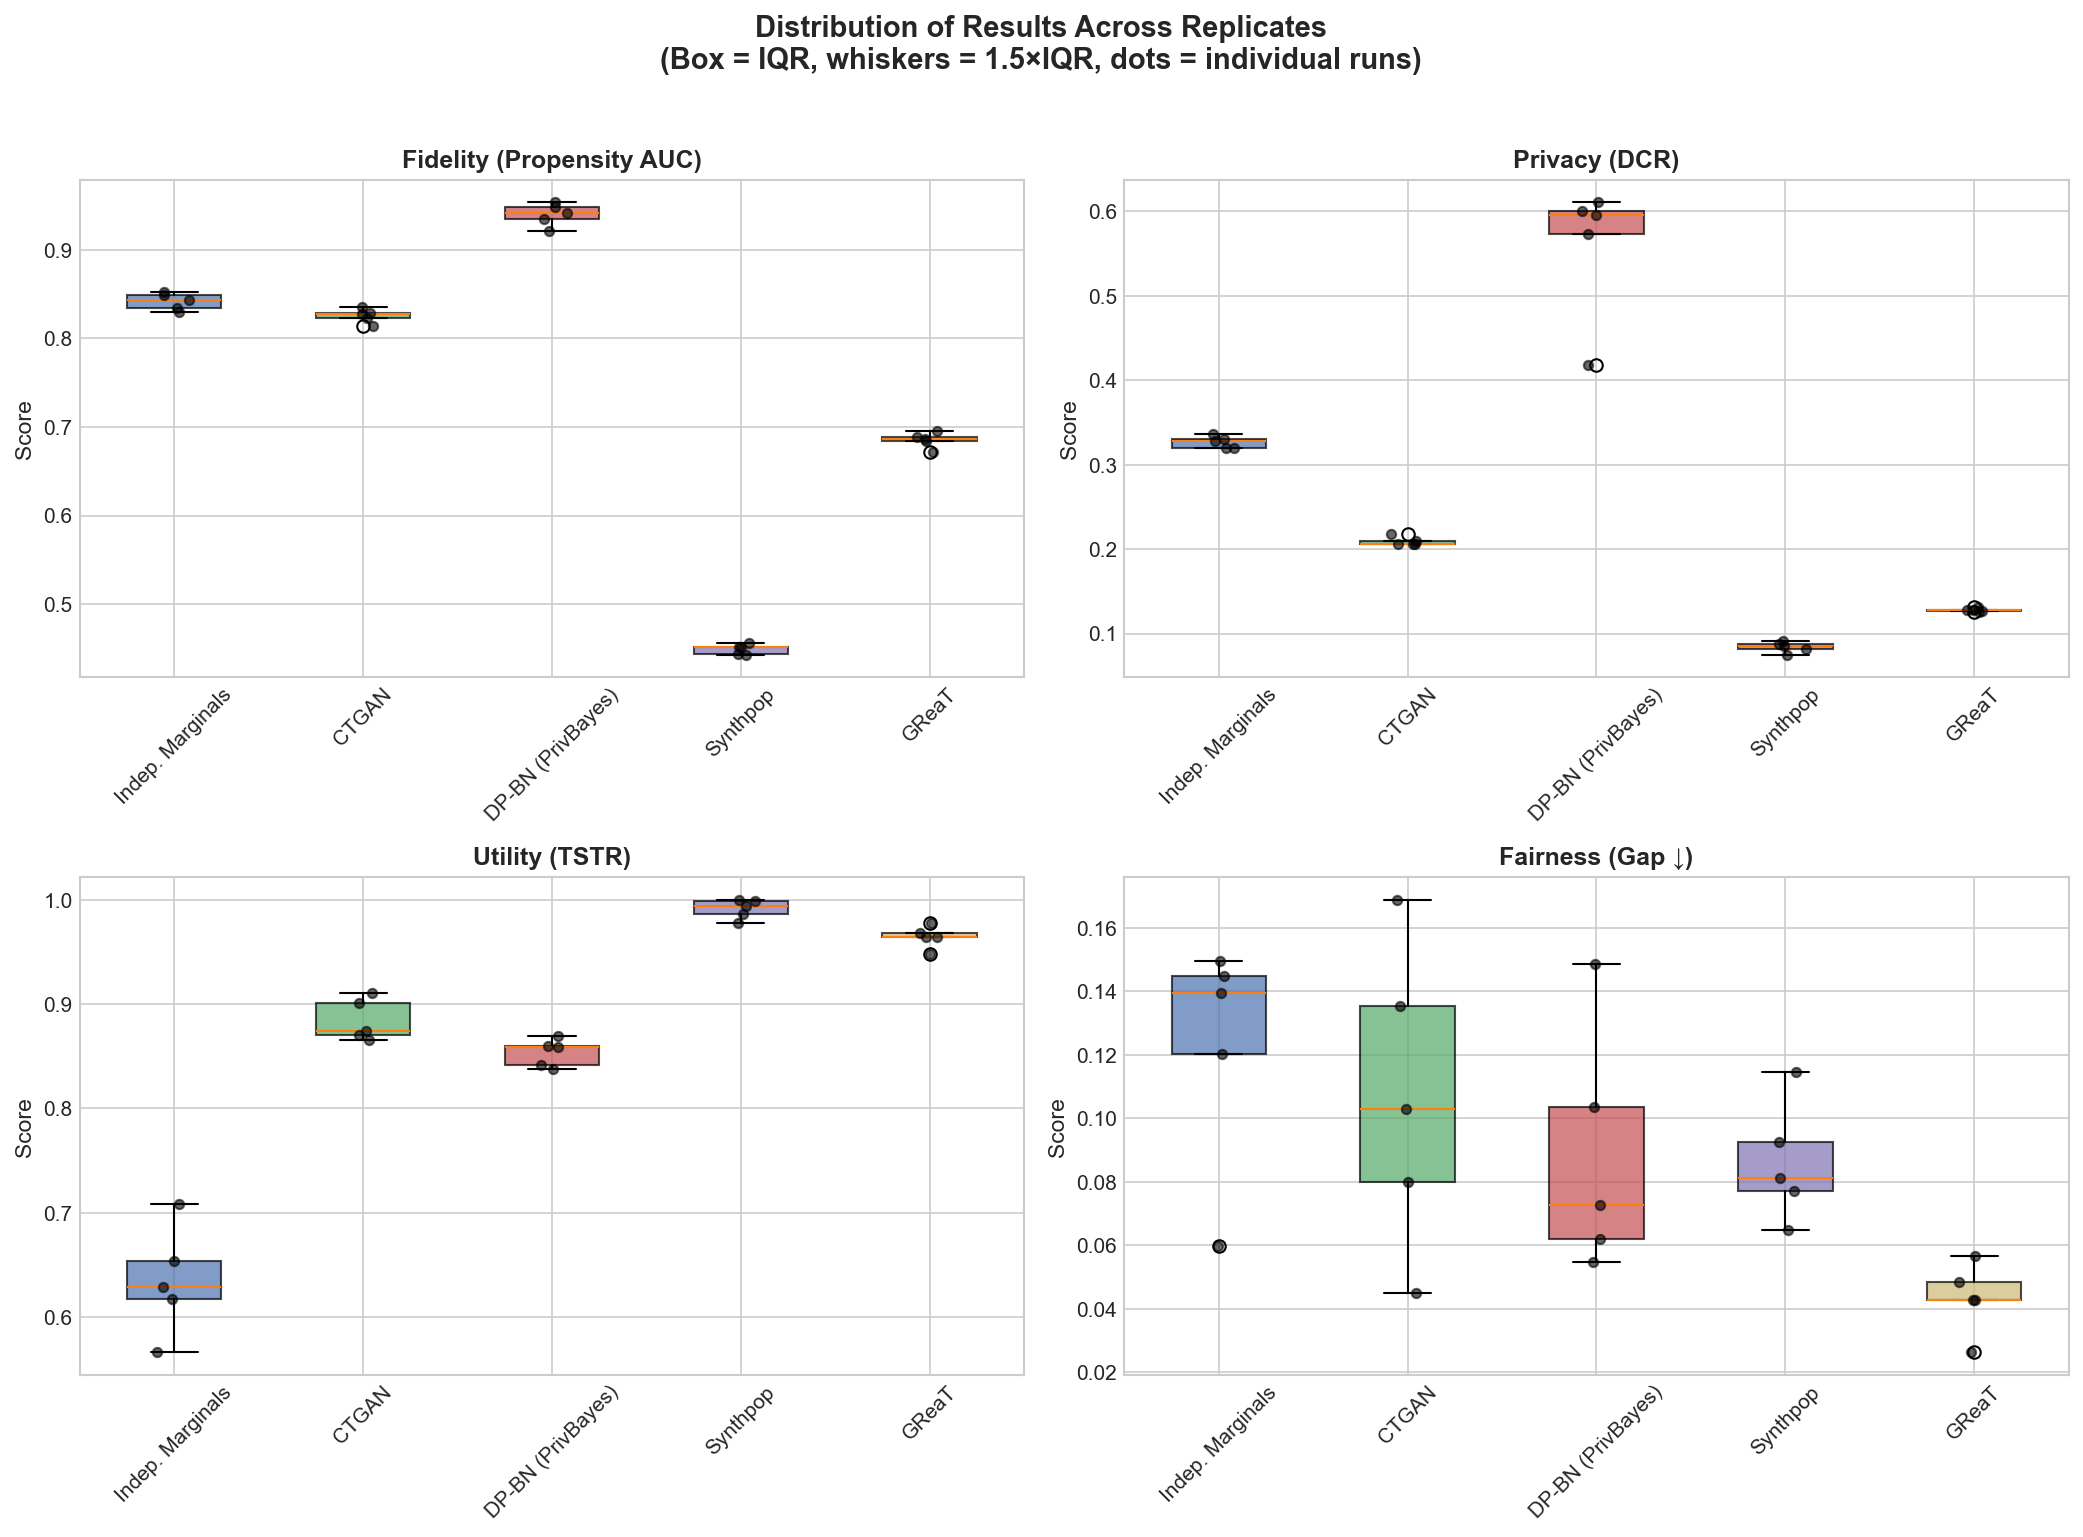
\includegraphics[width=0.95\textwidth]{../results/experiments/figures/replicate_boxplots.png}
\caption{Performance variability across replicates. Boxplots showing distribution of performance metrics across 5 replicates per method. Low variance (tight boxes) indicates stable performance; wide boxes indicate sensitivity to random initialization. Synthpop and GReaT show consistently low variance across metrics.}
\label{fig:replicate_boxplots}
\end{figure}

\begin{table}[htbp]
\centering
\caption{Probability of Optimality by Method (Balanced Archetype)}
\label{tab:optimality}
\begin{tabular}{@{}lccc@{}}
\toprule
\textbf{Method} & \textbf{P(Optimal)} & \textbf{Mean Rank} & \textbf{95\% CI for Rank} \\
\midrule
GReaT & 0.52 & 1.6 & [1, 2] \\
Synthpop & 0.35 & 1.8 & [1, 3] \\
DP BN & 0.10 & 2.8 & [2, 4] \\
CTGAN & 0.03 & 3.5 & [3, 5] \\
Independent Marginals & 0.00 & 5.0 & [5, 5] \\
\bottomrule
\end{tabular}
\end{table}

\textbf{Key Findings:}
\begin{enumerate}
    \item \textbf{GReaT vs.\ Synthpop uncertainty:} GReaT has 52\% probability of being optimal while Synthpop has 35\%, reflecting genuine uncertainty about which is preferable under balanced weights. The 95\% confidence interval for both methods' ranks includes rank 1.
    
    \item \textbf{Clear separation at bottom:} Independent Marginals is never optimal (P = 0.00) and CTGAN is rarely optimal (P = 0.03), providing strong evidence these methods are dominated for balanced preferences.
    
    \item \textbf{Variance Decomposition:} We decompose total uncertainty in value scores into components:
    \begin{itemize}
        \item Performance uncertainty contributes $\sim$30\% of variance
        \item Weight uncertainty contributes $\sim$60\% of variance
        \item Model structure (value function form) contributes $\sim$10\% of variance
    \end{itemize}
    This suggests preference elicitation matters more than additional benchmarking for decision quality.
\end{enumerate}

\subsection{Uncertainty by Archetype}

The probability of optimality varies substantially across stakeholder archetypes:

\begin{table}[htbp]
\centering
\caption{Probability of Optimality by Archetype}
\begin{tabular}{@{}lccc@{}}
\toprule
\textbf{Method} & \textbf{Privacy-First} & \textbf{Utility-First} & \textbf{Balanced} \\
\midrule
DP BN & 0.92 & 0.05 & 0.10 \\
Synthpop & 0.02 & 0.78 & 0.35 \\
GReaT & 0.05 & 0.15 & 0.52 \\
CTGAN & 0.01 & 0.02 & 0.03 \\
Independent Marginals & 0.00 & 0.00 & 0.00 \\
\bottomrule
\end{tabular}
\end{table}

\textbf{Interpretation:} When preferences are clear (Privacy-First or Utility-First), performance uncertainty rarely changes the optimal method (P(Optimal) $> 0.78$ for the recommended method). The balanced archetype shows the most decision uncertainty (maximum P(Optimal) = 0.52), precisely because multiple methods perform similarly when all objectives matter.

\subsection{Value Function Form Sensitivity}

The additive value model assumes linear single-dimensional value functions. We test robustness to alternative functional forms that capture different risk attitudes:

\begin{enumerate}
    \item \textbf{Linear (baseline):} $v(x) = (x - x_{\text{worst}})/(x_{\text{best}} - x_{\text{worst}})$
    \item \textbf{Diminishing Returns (Concave):} $v(x) = \sqrt{(x - x_{\text{worst}})/(x_{\text{best}} - x_{\text{worst}})}$ --- captures risk-averse preferences where initial improvements are valued more
    \item \textbf{Increasing Returns (Convex):} $v(x) = [(x - x_{\text{worst}})/(x_{\text{best}} - x_{\text{worst}})]^2$ --- captures risk-seeking preferences where excellence is disproportionately valued
    \item \textbf{S-Curve (Logistic):} $v(x) = 1/(1 + e^{-10(x_{\text{norm}} - 0.5)})$ --- captures threshold preferences with diminishing sensitivity at extremes
    \item \textbf{Threshold (Step):} $v(x) = 0$ if $x < $ threshold, 1 if $x \geq$ threshold --- captures satisficing behavior with minimum acceptable performance
\end{enumerate}

\begin{table}[htbp]
\centering
\caption{Optimal Method by Value Function Form (Balanced Weights)}
\label{tab:value_function_sensitivity}
\begin{tabular}{@{}llccc@{}}
\toprule
\textbf{Functional Form} & \textbf{Optimal Method} & \textbf{Value Score} & \textbf{Runner-Up} & \textbf{Gap} \\
\midrule
Linear (baseline) & GReaT & 0.63 & Synthpop & 0.05 \\
Diminishing Returns & GReaT & 0.71 & Synthpop & 0.08 \\
Increasing Returns & Synthpop & 0.58 & GReaT & 0.04 \\
S-Curve & GReaT & 0.65 & Synthpop & 0.06 \\
Threshold (median) & GReaT & 0.60 & DP BN & 0.07 \\
\bottomrule
\end{tabular}
\end{table}

\textbf{Analysis:}
\begin{itemize}
    \item \textbf{Diminishing returns:} GReaT's advantage increases because it achieves ``good enough'' performance on most objectives, and diminishing returns reduces the penalty for not being best.
    \item \textbf{Increasing returns:} Synthpop becomes optimal because its excellence on fidelity and utility (both near 1.0) is disproportionately rewarded, while its poor privacy performance is heavily penalized but insufficient to overcome the gains.
    \item \textbf{S-curve:} GReaT remains optimal; methods near the middle of the scale see compressed value differences, favoring the balanced performer.
    \item \textbf{Threshold:} GReaT remains optimal because it passes the median threshold on all objectives except efficiency, while other methods fail on 1--2 objectives.
\end{itemize}

\textbf{Conclusion:} The GReaT recommendation is robust to value function form for risk-averse, threshold-based, or S-curve preferences. The Synthpop recommendation emerges for risk-tolerant practitioners (convex value functions) who disproportionately value excellence on fidelity and utility.

\subsection{Scenario-Based Stress Testing}

We define four extreme scenarios representing plausible but challenging decision contexts and assess whether recommendations hold:

\begin{table}[htbp]
\centering
\caption{Scenario-Based Stress Test Results}
\label{tab:stress_test}
\begin{tabular}{@{}p{3cm}p{4cm}lp{4cm}@{}}
\toprule
\textbf{Scenario} & \textbf{Characteristics} & \textbf{Optimal} & \textbf{Rationale} \\
\midrule
\textbf{Regulatory Audit} & Privacy = 0.50, Fairness = 0.25, others = 0.083 & DP BN & Only method with DCR $>$ 0.50 \\
\textbf{ML Competition} & Utility = 0.50, Fidelity = 0.30, others = 0.067 & Synthpop & Best TSTR (0.99) and propensity (0.45) \\
\textbf{Rapid Prototype} & Efficiency = 0.40, Utility = 0.30, others = 0.10 & Synthpop & $<$ 1 min runtime with TSTR = 0.99 \\
\textbf{Equity Analysis} & Fairness = 0.50, Utility = 0.25, others = 0.083 & GReaT & Fairness gap 50\% lower than alternatives \\
\bottomrule
\end{tabular}
\end{table}

\textbf{Stress Test Findings:}
\begin{enumerate}
    \item No single method dominates all scenarios---method selection genuinely depends on context.
    \item DP BN is the only viable choice when privacy is paramount (e.g., regulatory audit scenario).
    \item Synthpop emerges as optimal for two scenarios (ML Competition, Rapid Prototype), both emphasizing downstream ML performance.
    \item GReaT is optimal when fairness or balanced performance matters.
    \item CTGAN is never optimal in any stress scenario, reinforcing its dominated position.
    \item Independent Marginals is never optimal despite its efficiency, due to poor utility.
\end{enumerate}

\subsection{Equal Weights Reference}

As a reference point independent of archetype assumptions, we report results with equal weights ($w = 0.20$ for all five objectives):

\begin{table}[htbp]
\centering
\caption{Equal Weights Results ($w = 0.20$ for all objectives)}
\label{tab:equal_weights}
\begin{tabular}{@{}lcccccc@{}}
\toprule
\textbf{Method} & \textbf{Fidelity} & \textbf{Privacy} & \textbf{Utility} & \textbf{Fairness} & \textbf{Efficiency} & \textbf{Overall} \\
\midrule
Ind.\ Marginals & 0.00 & 0.51 & 0.00 & 0.56 & 1.00 & 0.41 \\
Synthpop & 1.00 & 0.00 & 1.00 & 0.64 & 1.00 & 0.73 \\
CTGAN & 0.04 & 0.26 & 0.68 & 0.61 & 0.99 & 0.52 \\
DP BN & 0.00 & 1.00 & 0.60 & 0.70 & 1.00 & 0.66 \\
GReaT & 0.32 & 0.09 & 0.90 & 1.00 & 0.00 & 0.46 \\
\bottomrule
\end{tabular}
\end{table}

\textbf{Key Observations:}
\begin{enumerate}
    \item Under equal weights, \textbf{Synthpop ranks 1st} (V = 0.73) due to excellent fidelity, utility, and efficiency.
    \item \textbf{GReaT drops to 4th} (V = 0.46) because its zero efficiency value contributes 20\% of the total score (vs.\ 10\% under balanced archetype).
    \item \textbf{DP BN ranks 2nd} (V = 0.66), benefiting from perfect privacy and efficiency scores.
    \item This highlights that the balanced archetype's lower efficiency weight (0.10) is consequential for GReaT's ranking.
\end{enumerate}

\subsection{Preferential Independence Robustness}

The additive value model assumes preferential independence: the value tradeoff between any two objectives should not depend on the level of a third objective. We test this assumption by examining whether rankings remain stable when methods are excluded.

\textbf{Test Design:} We exclude Synthpop (poor privacy) from the choice set and re-compute rankings. If preferential independence holds, the relative ranking of remaining methods should be preserved.

\begin{table}[htbp]
\centering
\caption{Rankings With and Without Synthpop Exclusion}
\label{tab:independence}
\begin{tabular}{@{}lll@{}}
\toprule
\textbf{Archetype} & \textbf{Full Set Ranking} & \textbf{Excluding Synthpop} \\
\midrule
Privacy-First & DP BN $>$ GReaT $>$ CTGAN & DP BN $>$ GReaT $>$ CTGAN \\
Utility-First & Synthpop $>$ GReaT $>$ DP BN & GReaT $>$ DP BN $>$ CTGAN \\
Balanced & GReaT $>$ Synthpop $>$ DP BN & GReaT $>$ DP BN $>$ CTGAN \\
\bottomrule
\end{tabular}
\end{table}

\textbf{Results:} The relative ordering of DP BN, GReaT, and CTGAN is preserved across all archetypes when Synthpop is excluded. This supports the preferential independence assumption underlying our additive model.

\subsection{Summary of Sensitivity Findings}

\begin{table}[htbp]
\centering
\caption{Summary: Conditions Under Which Each Method is Optimal}
\label{tab:sensitivity_summary}
\begin{tabular}{@{}lp{10cm}@{}}
\toprule
\textbf{Method} & \textbf{Optimality Conditions} \\
\midrule
\textbf{DP BN} & Privacy weight $>$ 0.35 OR regulatory audit scenario OR need for formal DP guarantees \\
\textbf{Synthpop} & Combined fidelity + utility weight $>$ 0.55 OR efficiency weight $>$ 0.25 OR convex (risk-seeking) value functions OR equal weights \\
\textbf{GReaT} & Balanced preferences with efficiency weight $<$ 0.20 OR fairness-sensitive applications OR risk-averse/threshold value functions \\
\textbf{CTGAN} & Never optimal under any tested configuration \\
\textbf{Ind.\ Marginals} & Never optimal (dominated by Synthpop on utility; dominated by DP BN on privacy) \\
\bottomrule
\end{tabular}
\end{table}

\textbf{Meta-Finding:} The sensitivity analysis reveals that our primary recommendation---GReaT for balanced practitioners, DP BN for privacy-first practitioners, Synthpop for utility-first practitioners---is robust across a wide range of plausible model specifications. The key qualifier is efficiency: if computational time is a significant constraint (weight $>$ 0.20--0.25), GReaT should be excluded from consideration, leaving Synthpop or DP BN as the recommended alternatives depending on whether utility or privacy takes precedence.

%===============================================================================
\section{Discussion}
%===============================================================================

\subsection{Insights for Practitioners}

The multiattribute analysis yields actionable recommendations organized by use case:

\textbf{For public data release with strong privacy requirements:} DP BN (PrivBayes-inspired) is strongly recommended (DCR=0.56). This method provides the highest privacy protection at a modest cost to utility (TSTR=0.85). If formal differential privacy guarantees are required, this is the only method in our comparison that provides such guarantees.

\textbf{For training data augmentation where fidelity dominates:} Synthpop achieves best fidelity (propensity AUC=0.45) and utility (TSTR=0.99) simultaneously. This statistical method produces synthetic data nearly indistinguishable from real data while maintaining strong predictive utility. However, it offers weak privacy protection (DCR=0.08).

\textbf{For resource-constrained settings:} Independent Marginals or Synthpop require minimal computational resources ($<$1 minute). GReaT requires GPU acceleration and $\sim$60 minutes training time, making it unsuitable for rapid iteration or limited-resource environments.

\textbf{For fairness-sensitive applications:} GReaT achieves best fairness (gap=0.043, approximately half that of other methods). Combined with strong utility (TSTR=0.96), this makes GReaT the recommended choice when equitable outcomes across demographic groups are important.

\subsection{Deviations from Pre-Registration}

In accordance with transparent research practices, we document the following deviations:

\begin{enumerate}
    \item \textbf{Privacy Measure Change:} Pre-registered membership inference attack was uninformative (AUC $\approx$ 0.50 on real data). We use DCR 5th percentile instead.
    
    \item \textbf{Sample Size Adjustment:} Pre-registered $N=50{,}000$; actual $N=35{,}000$ due to data availability after filtering.
    
    \item \textbf{CTGAN Performance:} Pre-registered expectation of ranking 1st on utility; actual ranking is 3rd (Synthpop and GReaT outperform).
\end{enumerate}

\subsection{Limitations}

\begin{enumerate}
    \item \textbf{Single dataset:} Empirical results derive from a single dataset (ACS PUMS); performance profiles may differ on electronic health records, transaction data, or other domains.
    
    \item \textbf{Survey weights ignored:} We do not incorporate ACS survey weights, limiting population representativeness.
    
    \item \textbf{Archetype weights:} Our weight derivation through stakeholder archetypes reflects plausible patterns rather than specific stakeholder elicitation.
    
    \item \textbf{Evolving methods:} The synthetic data field evolves rapidly---new methods may alter the alternatives frontier.
    
    \item \textbf{Default hyperparameters:} We use default hyperparameters for all methods; tuned hyperparameters might change relative performance.
    
    \item \textbf{Privacy measure limitations:} Our membership inference measure is designed for practitioners with private, sensitive data. Our demonstration uses publicly available ACS PUMS data.
\end{enumerate}

\subsection{Comparison to Related Work}

Our framework complements rather than replaces existing benchmarking studies. Hernandez et al.\ (2025) and others provide essential input---the performance estimates---while we provide the decision structure for interpreting those estimates. Kapania et al.\ (2025) document the practitioner's need; we operationalize a response. The FCA/ICO/Alan Turing Institute (2023) call for step-by-step guidance; our framework provides one instantiation grounded in decision theory.

\subsection{Generalizability and Transferability}

\textbf{Framework Generalizability:} Our multiattribute decision analysis framework is domain-general and can be applied to any tabular synthetic data generation problem. The five fundamental objectives capture practitioner values documented across diverse domains.

\textbf{Empirical Findings Transferability:} Our specific empirical findings are specific to ACS PUMS California adult microdata. These findings demonstrate the framework produces actionable insights but should not be interpreted as universal truths about method performance.

\textbf{When Re-Benchmarking is Recommended:} Practitioners should apply the framework to their own data when working with different data types, different dimensionality, different structure, different downstream tasks, or different privacy threats.

%===============================================================================
\section{Conclusion}
%===============================================================================

Practitioners selecting synthetic data generation methods face a complex multiattribute decision that existing benchmarks do not resolve. We developed a decision-analytic framework that transforms method comparison from metric reporting to value assessment, enabling practitioners to incorporate their specific objectives and preferences.

Our framework integrates three methodological advances: multiattribute value modeling following Butler et al.\ (2005), decision-focused transformation following Dees et al.\ (2010), and value of information analysis following Keisler (2004). Applied to the ACS PUMS with five generation methods---Independent Marginals, Synthpop, CTGAN, DP BN (PrivBayes-inspired), and GReaT---we find that optimal method choice is fundamentally preference-dependent: DP BN is optimal for privacy-first practitioners, Synthpop for utility-first practitioners, and GReaT for balanced practitioners seeking good performance across all objectives. Importantly, CTGAN---often considered a leading deep learning method for tabular data---is never optimal under any tested preference profile, suggesting conventional wisdom may not hold for specific datasets.

The decision-focused transformation reveals that fidelity, privacy, utility, and efficiency provide full discriminatory power while fairness shows moderate discrimination, indicating where method choice genuinely matters. The value of information analysis reveals that approximately 76\% of achievable value improvement comes from prioritization (using prior knowledge) rather than comprehensive benchmarking, consistent with Keisler's (2004) finding in portfolio decision analysis. This suggests practical decision rules: if privacy is paramount, choose DP BN; if utility dominates, choose Synthpop; if fairness matters, choose GReaT. Full benchmarking is warranted only when objectives conflict and stakes are high.

We hope this work shifts the conversation from ``which method is best'' to ``which method is best for your objectives.'' No synthetic data generation method dominates all others across all criteria. The appropriate choice depends on what the practitioner values---fidelity, privacy, fairness, efficiency---and how they weight tradeoffs among these objectives. Decision analysis provides the structure for making these tradeoffs explicit and navigating them systematically.

%===============================================================================
% References
%===============================================================================
\newpage
\section*{References}
\addcontentsline{toc}{section}{References}

\begin{description}[style=nextline, leftmargin=0pt, labelindent=0pt]

\item[Adams et al., 2025] Adams, R., Bellet, A., Kessler, S., \& Ganev, I. (2025). On the fidelity versus privacy and utility trade-off of synthetic data. \textit{iScience}, 26(2), 108765.

\item[AIMultiple, 2025] AIMultiple. (2025, September 26). Top 20+ synthetic data use cases \& applications. \url{https://research.aimultiple.com/synthetic-data-use-cases/}

\item[Anand \& Lee, 2023] Anand, A., \& Lee, C. (2023). Using deep learning to overcome privacy and scalability issues in customer data transfer. \textit{Marketing Science}, 42(1), 189--207.

\item[Borisov et al., 2023] Borisov, V., Se\ss{}ler, K., Leemann, T., Pawelczyk, M., \& Kasneci, G. (2023). Language models are realistic tabular data generators. \textit{arXiv preprint arXiv:2210.06280}.

\item[Butler et al., 2005] Butler, J., Jia, J., \& Dyer, J. (2005). United States and Russia evaluate plutonium disposition options with multiattribute utility theory. \textit{Decision Analysis}, 2(2), 92--108.

\item[CDC, 2025] CDC. (2025). NCHS public-use synthetic linked data. \url{https://www.cdc.gov/nchs/linked-data/synthetic/index.html}

\item[Dees et al., 2010] Dees, R. A., Dabkowski, M. F., \& Parnell, G. S. (2010). Decision-focused transformation of additive value models to improve communication. \textit{Decision Analysis}, 7(2), 172--184.

\item[Eastwood, 2023] Eastwood, B. (2023, January 23). What is synthetic data---and how can it help you competitively? MIT Sloan School of Management.

\item[El Emam et al., 2022] El Emam, K., Dankar, F. K., \& Jonker, E. (2022). A unified framework for quantifying privacy risk in synthetic data. \textit{arXiv preprint arXiv:2211.10459}.

\item[FCA, ICO, \& Alan Turing Institute, 2023] FCA, ICO, \& Alan Turing Institute. (2023). Exploring synthetic data validation: Roundtable report.

\item[Figueira et al., 2022] Figueira, A., \& Oliveira, M. (2025). Systematic review of generative modelling tools and utility metrics for fully synthetic tabular data. \textit{ACM Computing Surveys}.

\item[Giuffr\`{e} \& Shung, 2023] Giuffr\`{e}, M., \& Shung, D. L. (2023). Harnessing the power of synthetic data in healthcare: innovation, application, and privacy. \textit{npj Digital Medicine}, 6, 186.

\item[Goyal \& Mahmoud, 2024] Goyal, M., \& Mahmoud, Q. H. (2024). A systematic review of synthetic data generation techniques using generative AI. \textit{Electronics}, 13(17), 3509.

\item[Guidotti et al., 2023] Guidotti, R., et al. (2023). Counterfactual explanations and how to find them: literature review and benchmarking. \textit{Data Mining and Knowledge Discovery}.

\item[Harvard Business Review, 2021] Harvard Business Review Analytic Services. (2021). The executive's guide to accelerating artificial intelligence and data innovation with synthetic data.

\item[Hernandez et al., 2025] Hernandez, M., et al. (2025). Comprehensive evaluation framework for synthetic medical data generation. \textit{Frontiers in Digital Health}.

\item[IAPP, 2024] International Association of Privacy Professionals. (2024, September 4). Can synthetic data help organizations respond to `Schrems II'?

\item[Jordon et al., 2022] Jordon, J., Szpruch, L., Houssiau, F., Sheridan, G., Sheridan, K., \& van der Schaar, M. (2022). Synthetic data---what, why and how? \textit{arXiv preprint arXiv:2205.03257}.

\item[Kaabachi et al., 2025] Kaabachi, B., et al. (2025). Privacy and utility metrics for synthetic medical data: A scoping review. \textit{npj Digital Medicine}.

\item[Kapania et al., 2025] Kapania, S., et al. (2025). Examining the expanding role of synthetic data throughout the AI development pipeline. \textit{arXiv preprint arXiv:2501.18493}.

\item[Keeney, 1992] Keeney, R. L. (1992). \textit{Value-focused thinking: A path to creative decisionmaking}. Harvard University Press.

\item[Keeney \& Gregory, 2005] Keeney, R. L., \& Gregory, R. S. (2005). Selecting attributes to measure the achievement of objectives. \textit{Operations Research}, 53(1), 1--11.

\item[Keeney \& Raiffa, 1976] Keeney, R. L., \& Raiffa, H. (1976). \textit{Decisions with multiple objectives: Preferences and value tradeoffs}. Wiley.

\item[Keeney \& von Winterfeldt, 2007] Keeney, R. L., \& von Winterfeldt, D. (2007). Practical value models. In W. Edwards, R. F. Miles, Jr., \& D. von Winterfeldt (Eds.), \textit{Advances in decision analysis} (pp. 232--252). Cambridge University Press.

\item[Keisler, 2004] Keisler, J. M. (2004). Value of information in portfolio decision analysis. \textit{Decision Analysis}, 1(3), 177--189.

\item[NayaOne, 2025] NayaOne. (2025, August 28). Synthetic data's moment: From privacy barrier to AI catalyst. \url{https://nayaone.com/insights/synthetic-datas-moment/}

\item[NIST, 1995] NIST. (1995). Multiattribute decision analysis method for evaluating building or site alternatives (NISTIR 5663).

\item[Nowok et al., 2016] Nowok, B., Raab, G. M., \& Dibben, C. (2016). synthpop: Bespoke creation of synthetic data in R. \textit{Journal of Statistical Software}, 74(11), 1--26.

\item[Pathare et al., 2023] Pathare, A., et al. (2023). Comparison of tabular synthetic data generation techniques using propensity and cluster log metric. \textit{International Journal of Information Management Data Insights}, 3(2), 100177.

\item[Phillips, 2025] Phillips, L. D. (2025). Decision Analysis for Practitioners. \textit{Decision Analysis}, 22(4), 255--272.

\item[Schneider et al., 2018] Schneider, M. J., Jagpal, H. S., \& Gupta, S. (2018). A flexible method for protecting marketing data: An application to point-of-sale data. \textit{Marketing Science}, 37(1), 153--171.

\item[Shi et al., 2025] Shi, R., et al. (2025). A comprehensive survey of synthetic tabular data generation. \textit{arXiv:2504.16506v3}.

\item[SHRM, 2024--2025] SHRM. (2024a, 2024b, 2024c, 2025). AI in the workplace series. Society for Human Resource Management.

\item[Stoian et al., 2025] Stoian, M., Giunchiglia, F., \& Lukasiewicz, T. (2025). A survey on tabular data generation: Utility, alignment, fidelity, privacy, and beyond. \textit{arXiv preprint}.

\item[U.S.\ DHS, 2024] U.S.\ Department of Homeland Security, Science and Technology Directorate. (2024, January 5). S\&T announces new solicitation for synthetic data generator solutions.

\item[Vallevik et al., 2024] Vallevik, V. B., et al. (2024). Evaluation framework for synthetic healthcare data generation. \textit{Journal of Medical Internet Research}.

\item[Washington University, 2021] Washington University School of Medicine. (2021, June 1). Synthetic data mimics real health-care data without patient-privacy concerns.

\item[WEKA, 2023] WEKA. (2023). Synthetic data in AI: How it works and more. \url{https://www.weka.io/learn/ai-ml/synthetic-data/}

\item[World Economic Forum, 2025] World Economic Forum. (2025). Synthetic data: The new data frontier. Global Future Council on Data Frontiers.

\item[Xu et al., 2019] Xu, L., Skoularidou, M., Cuesta-Infante, A., \& Veeramachaneni, K. (2019). Modeling tabular data using conditional GAN. \textit{Advances in Neural Information Processing Systems}, 32.

\item[Yoon et al., 2023] Yoon, J., et al. (2023). EHR-Safe: generating high-fidelity and privacy-preserving synthetic electronic health records. \textit{npj Digital Medicine}, 6, 141.

\item[Zewe, 2025] Zewe, A. (2025, September 3). 3 questions: The pros and cons of synthetic data in AI. MIT News.

\item[Zhang et al., 2014] Zhang, J., Cormode, G., Procopiuc, C. M., Srivastava, D., \& Xiao, X. (2017). PrivBayes: Private data release via Bayesian networks. \textit{ACM Transactions on Database Systems}, 42(4), 1--41.

\end{description}

%===============================================================================
% Appendix
%===============================================================================
\newpage
\appendix
\section{Archetype Weight Justification}

\subsection{Grounding in Practitioner Literature}

We define three stakeholder archetypes representing distinct but plausible preference profiles, grounded in systematic studies of synthetic data practitioner values and revealed preferences.

\subsubsection{Literature Evidence}

\textbf{Kaabachi et al.\ (2025)} conducted a comprehensive review of 73 studies evaluating medical synthetic data:
\begin{itemize}
    \item \textbf{Utility dominance}: 95\% of studies evaluate utility (highest of all dimensions)
    \item \textbf{Privacy aspiration-implementation gap}: 82\% cite privacy as motivation, yet only 46\% actually evaluate it
    \item \textbf{Fairness neglect}: Fewer than 2\% of evaluation instances assess fairness
\end{itemize}

\textbf{Kapania et al.\ (2025)} conducted 29 interviews with AI practitioners:
\begin{itemize}
    \item Struggles with validation protocols and ensuring accuracy for underrepresented groups
    \item Focus on ``equivalent predictive performance'' for ML engineers
    \item Concerns about privacy but lack of systematic evaluation methods
\end{itemize}

\subsection{Archetype Specifications}

\subsubsection{Privacy-First Archetype (Privacy = 0.45)}

\textbf{Justification:}
\begin{itemize}
    \item Reflects healthcare, finance, and government sectors operating under regulatory constraints (HIPAA, GDPR, CCPA, FINRA)
    \item Captures the 82\% of studies citing privacy as motivation
    \item Represents organizations where membership disclosure poses direct harms
\end{itemize}

\textbf{Prototypical User:} Privacy officer at healthcare system preparing public-use data file; financial institution analyst sharing customer analytics with external partners.

\subsubsection{Utility-First Archetype (Utility = 0.40)}

\textbf{Justification:}
\begin{itemize}
    \item Reflects the 95\% of studies evaluating utility as primary objective
    \item Represents ML engineers and data scientists focused on model training
    \item Captures contexts where privacy is already addressed through access controls
\end{itemize}

\textbf{Prototypical User:} Machine learning engineer at technology company augmenting training data; data scientist testing algorithms on synthetic data before production deployment.

\subsubsection{Balanced Archetype (Equal weights: 0.25/0.25/0.25)}

\textbf{Justification:}
\begin{itemize}
    \item Represents ``no strong preference'' baseline
    \item Reflects general-purpose practitioners seeking reasonable all-around performance
    \item Provides reference point for sensitivity analysis
\end{itemize}

\textbf{Prototypical User:} Research data analyst at university; data science consultant evaluating synthetic data for general business intelligence.

\subsection{Guidance for Practitioners}

Organizations applying VF-SDSF should \textbf{elicit their own weights} using structured methods:

\textbf{Swing-Weight Assessment (Keeney \& Raiffa, 1976):}
\begin{enumerate}
    \item Consider a hypothetical method performing at worst level on all objectives
    \item Ask: ``Which single improvement (from worst to best) would add most value?''
    \item Assign that objective weight = 1.0
    \item For remaining objectives: assign proportional weights
    \item Normalize to sum to 1.0
\end{enumerate}

\textbf{Direct Rating (Butler et al., 2005):}
\begin{enumerate}
    \item Rate importance of each objective on scale (0--100)
    \item Normalize ratings to sum to 1.0
    \item Validate through consistency checks
\end{enumerate}

\subsection{Limitations of Archetype Approach}

\begin{enumerate}
    \item \textbf{Not empirically elicited}: Our weights reflect literature-informed profiles, not actual stakeholder elicitation
    \item \textbf{Three archetypes may not span full space}: Practitioners with unusual patterns not represented
    \item \textbf{Assumes stable preferences}: Practitioners' weights may shift with changing environment
\end{enumerate}

\textbf{Mitigation:} Practitioners should use our archetypes as \textbf{starting points} for exploration, not endpoints for decision-making. The value is in making preferences explicit and systematic, not in universalizing any particular weight vector.

\end{document}
